\documentclass[12pt,a4paper,oneside]{book}

\usepackage{mystyle}

\title{A First Course in Graph Theory}
\author{Gary Chartrand, Ping Zhang}
\date{Spring 2016}

\begin{document}
\parindent 15pt

\frontmatter
\maketitle
\tableofcontents
\chapter{Preface}
Perhaps it's not so surprising that when we (the authors) were learning mathematics, we thought that we were being taught some well-known facts -- facts that had been around forever. It wasn't until later that we started to understand that these facts (the word "theorem" was beginning to become part of our vocabulary) had not been around forever and that \it{people} had actually discovered these facts. Indeed, \it{names} of people were becoming part of the discussion.

Mathematics has existed for many centuries. In the ancient past, certain cultures developed their own mathematics. This was certainly the case with Egypt, Babylonia, Greece, China, India and Japan. In recent centuries, there has become only one international mathematics. It has become more organized and has been divided into more clearly defined areas (even though there is significant overlap). While this was occurring, explanations (proofs) as to why mathematical statements are true were becoming more structured and clearly written.

The goal of this book is to introduce undergraduates to the mathematical area called \it{graph theory}, which only came into existence during the first half of the 18th century. This area didn't start to develop into an organized branch of mathematics until the second half of the 19th century and there wasn't even a book on the subject until the first half of the 20th century. Since the second half of the 20th century, however, the subject has exploded.

It is our intent to describe some of the major topics of this subject to you and to inform you of some of the people who helped develop and shape this area. In the beginning, most of these people were just like you -- students who enjoyed mathematics but with a great sense of curiosity. As with everything else (though not as often talked about), mathematics has its non-serious side and we've described some of this as well. Even the most brilliant mathematicians don't know everything and we've presented some topics that have not been well-studied and in which the answers (and even the questions) are not known. This will give you the chance to do some creative thinking of your own. In fact, maybe the next person who will have an influence on this subject is you.

Part of what makes graph theory interesting is that graphs can be used to model situations that occur within certain kinds of problems. These problems can then be studied (and possibly solved) with the aid of graphs. Because of this, graph models occur frequently throughout this textbook. However, graph theory is an area of mathematics and consequently concerns the study of mathematical ideas -- of concepts and their connections with each other. The topics and result we have included were chosen because we feel they are interesting, important and/or are representative of the subject.

As we said, this text has been written for undergraduates. Keeping this in mind, we have included a proof of a theorem if we believe it is appropriate, the proof technique is informative and if the proof is not excessively long. We would like to think that the material in this text will be useful and interesting for mathematics students as well as for other students whose areas of interest include graphs. This text is also appropriate for self-study.

We have included three appendixes. In Appendix A, we review some important facts about sets and logic. Appendix B is devoted to equivalence relations and functions while Appendix 3 describes methods of proof. We understand how frustrating it is for students (or anyone!) who try to read a proof that is not reader-friendly and which leaves too many details for the reader to supply. Consequently, we have endeavored to give clear, well-written proofs.

Although this can very well be said about any area of mathematics or indeed about any scholarly activity, we feel that appreciation of graph theory is enhanced by being familiar with many of the people, past and present, who were or are responsible for its development. Consequently, we have included several remarks that we find interesting about some of the "people of graph theory." Since we believe that these people are part of the story that is graph theory, we have discussed them within the text and not simply as footnotes. We often fail to recognize that mathematics is a living subject. Graph theory was created by \it{people} and is a subject that is still evolving.

There are several sections that have been designated as "Excursion." These can be omitted with no negative effect if this text is being used for a course. In some cases, an Excursion is an area of graph theory we find interesting but which the instructor may choose not to discuss due to lack of time or because it's not one of his or her favorites. In other cases, an Excursion brings up a sidelight of graph theory that perhaps has little, if any, mathematical content but which we simply believe is interesting.

There are also sections that we have designated as "Exploration." These sections contain topics with which students can experiment and use their imagination. These give students opportunities to practice asking questions. In any case, we believe that this might be fun for some students.

As far as using this text for a course, we consider the first three chapters as introductory. Much of this could be covered quite quickly. Students could read these chapters on their own. It isn't necessary to cover connectivity and Menger's Theorem if the instructor chooses not to do so. Sections 8.3, 9.2, 10.3 and 11.2 could easily be omitted, while material from Chapters 12 and 13 can be covered according to the instructor's interest.

Solutions or hints for the odd-numbered exercises in the regular sections of the text, references, an index of mathematical terms, an index of people and a list of symbols are provided at the end of the text.

It was because of discussions we had with Robert Ross that we decided to write "An Introduction to Graph Theory." We thank him for this and for his encouragement. We especially that John Grafton, Senior Reprint Editor at Dover Publications, whose encouragement led us to revise the book, with its new title "A First Course in Graph Theory." We are most grateful to the reviewers of the original edition who gave us many valuable suggestions: Jay Bagga, Ball State University; Richard Borie, University of Alabama; Anthony Evans, Wright State University; Mark Ginn, Appalachian State University; Mark Goldberg, Rensselaer Polytechnic Institute; Arthur Hobbs, Texas A\&M University; Garth Isaak, Lehigh University; Daphne Liu, California State University, Los Angeles; Alan Mills, Tennessee Technological University; Dan Pritikin, Miami University; John Reay, Western Washington University; Yue Zhao, University of Central Florida.

\begin{flushright}
Gary Chartrand and Ping Zhang\\
May 2011
\end{flushright}

\mainmatter
\chapter{Introduction}
\section{Graphs and Graph Models}
A major publishing company has ten editors (referred to by 1, 2,\ldots, 10) in the scientific, technical and computing areas. These ten editors have a standard meeting time during the first Friday of every month and have divided themselves into seven committees to meet later in the day to discuss specific topics of interest to the company, namely, advertising, securing reviewers, contacting new potential authors, finances, used and rented copies, electronic editions and competing textbooks. This leads us to our first example.

\begin{exmp}
The ten editors have decided on the seven committees: $c_{1}$ = \{1,2,3\}, $c_{2}$ = \{1,3,4,5\}, $c_{3}$ = \{2,5,6,7\}, $c_{4}$ = \{4,7,8,9\}, $c_{5}$ = \{2,6,7\}, $c_{6}$ = \{8,9,10\}, $c_{7}$ = \{1,3,9,10\}. They have set aside three time periods for the seven committees to meet on those Fridays when all ten editors are present. Some pairs of committees cannot meet during the same period because one or two of the editors are on both committees. This situation can be modeled visually as shown in Figure 1.1.

\begin{figure}[h]
	\[G:
	\raisebox{-.5\height}
	{
		\begin{tikzpicture}[x=1.5cm, y=1.5cm]
			\foreach \i/\j in {0/1, -1/2, 5/3, 4/4, 3/5, 2/6, 1/7} {
				\setcounter{Angle}{90 + \i * 360 / 7};
				\vertex (c\j) at (\theAngle:1) [label=\theAngle:$c_{\j}$]{};
			}
			\path
				(c1) edge (c2)
				(c1) edge (c3)
				(c1) edge (c5)
				(c1) edge (c7)
				(c2) edge (c3)
				(c2) edge (c4)
				(c2) edge (c7)
				(c3) edge (c4)
				(c3) edge (c5)
				(c4) edge (c5)
				(c4) edge (c6)
				(c4) edge (c7)
				(c6) edge (c7)
			;
		\end{tikzpicture}
	}\]
	\caption{A graph}
\end{figure}

In this figure, there are seven small circles, representing the seven committees and a straight line segment is drawn between two circles if the committees they represent have at least one committee member in common. In other words, a straight line segment between two small circles (committees) tells us that these two committees should not be scheduled to meet at the same time. This gives us a picture or a "model" of the committees and the overlapping nature of their membership.
\end{exmp}

What we have drawn in Figure 1.1 is called a graph. Formally, a \bf{graph} $G$ consists of a finite nonempty set $V$ of objects called \bf{vertices} (the singular is \bf{vertex}) and a set $E$ of 2-element subsets of $V$ called \bf{edges}. The sets $V$ and $E$ are the \bf{vertex set} and \bf{edge set} of $G$, respectively. So a graph $G$ is a pair (actually an \it{ordered} pair) of two sets $V$ and $E$. For this reason, some write $G = (V,E)$. At times, it is useful to write $V(G)$ and $E(G)$ rather than $V$ and $E$ to emphasize that these are the vertex and edge sets of a particular graph $G$. Although $G$ is the common symbol to use for a graph, we also use $F$ and $H$, as well as $G'$, $G''$ and $G_{1}$, $G_{2}$, etc. Vertices are sometimes called \bf{points} or \bf{nodes} and edges are sometimes called \bf{lines}. Indeed, there are some who use the term \bf{simple graph} for what we call a graph. Two graphs $G$ and $H$ are \bf{equal} if $V(G) = V(H)$ and $E(G) = E(H)$, in which case we write $G = H$.

It is common to represent a graph by a diagram in the plane (as we did in Figure 1.1) where the vertices are represented by points (actually small circles -- open or solid) and whose edges are indicated by the presence of a line segment or curve between the two points in the plane corresponding to the appropriate vertices. The diagram itself is then also referred to as a graph. For the graph $G$ of Figure 1.1 then, the vertex set of $G$ is $V(G) = \{c_{1},c_{2},\ldots,c_{7}\}$ and the edge set of $G$ is
\begin{align*}
E(G) = &\{\{c_{1},c_{2}\},\{c_{1},c_{3}\},\{c_{1},c_{5}\},\{c_{1},c_{7}\},\{c_{2},c_{3}\},\{c_{2},c_{4}\},\{c_{2},c_{7}\},\\
&\{c_{3},c_{4}\},\{c_{3},c_{5}\},\{c_{4},c_{5}\},\{c_{4},c_{6}\},\{c_{6},c_{7}\}\}.
\end{align*}

Let's consider another situation. Have you ever encountered this sequence of integers before?
\begin{align*}
1, 1, 2, 3, 5, 8, 13, 21, 34, 55, \ldots
\end{align*}
Every integer in the sequence is the sum of the two integers immediately preceding it (except for the first two integers of course). These numbers are well known in mathematics and are called the \bf{Fibonacci numbers}. In fact, these integers occur so often that there is a journal (\it{The Fibonacci Quarterly}, frequently published \it{five} times a year!) devoted to the study of their properties. Our second example concerns these numbers.

\begin{exmp}
Consider the set $S$ = \{2,3,5,8,13,21\} of six specific Fibonacci numbers. There are some pairs of distinct integers belonging to $S$ whose sum or difference (in absolute value) also belongs to $S$, namely, \{2,3\}, \{2,5\}, \{3,5\}, \{3,8\}, \{5,8\}, \{5,13\}, \{8,13\}, \{8,21\} and \{13,21\}. There is a more visual way of identifying these pairs, namely by the graph $H$ of Figure 1.2. In this case, $V(H) = \{2,3,5,8,13,21\}$ and
\begin{align*}
E(H) = \{\{2,3\},\{2,5\},\{3,5\},\{3,8\},\{5,8\},\{5,13\},\{8,13\},\{8,21\},\{13,21\}\}.
\end{align*}
\end{exmp}

\begin{figure}[h]
	\[H:
	\raisebox{-.5\height}
	{
		\begin{tikzpicture}[x=1.5cm, y=1.5cm]
			\foreach \i/\j in {1/2, 0/3, 5/5, 4/8, 3/13, 2/21} {
				\setcounter{Angle}{\i * 360 / 6};
				\vertex (\j) at (\theAngle:1) [label=\theAngle:$\j$]{};
			}
			\path
				(2) edge (3)
				(2) edge (5)
				(3) edge (5)
				(3) edge (8)
				(5) edge (8)
				(5) edge (13)
				(8) edge (13)
				(8) edge (21)
				(13) edge (21)
			;
		\end{tikzpicture}
	}\]
	\caption{Another graph}
\end{figure}

When dealing with graphs, it is customary and simpler to represent an edge $\{u,v\}$ by $uv$ (or $vu$). If $uv$ is an edge of $G$, then $u$ and $v$ are said to be \bf{adjacent} in $G$. The number of vertices in $G$ is often called the \bf{order} of $G$, while the number of edges is its \bf{size}. Since the vertex set of every graph is nonempty, the order of every graph is at least 1. A graph with exactly one vertex is called a \bf{trivial graph}, implying that the order of a \bf{nontrivial graph} is at least 2. The graph $G$ of Figure 1.1 has order 7 and size 13, while the graph $H$ of Figure 1.2 has order 6 and size 9. We often use $n$ and $m$ for the order and size, respectively, of a graph. So, for the graph $G$ of Figure 1.1, $n = 7$ and $m = 13$; while for the graph $H$ of Figure 1.2, $n = 6$ and $m = 9$.

A graph $G$ with $V(G) = \{u,v,w,x,y\}$ and $E(G) = \{uv,uw,vw,vx,wx,xy\}$ is shown in Figure 1.3(a). There are occasions when we are interested in the structure of a graph and not in what the vertices are called. In this case, a graph is drawn without labeling its vertices. For this reason, the graph $G$ of Figure 1.3(a) is a \bf{labeled graph} and Figure 1.3(b) represents an \bf{unlabeled graph}.

\begin{figure}[h]
	\centering
	\begin{subfigure}[b]{.4\textwidth}
		\[G:
		\raisebox{-.5\height}
		{
			\begin{tikzpicture}[x=1.5cm, y=1.5cm]
				\vertex (u) at (90:1) [label=above:$u$]{};
				\vertex (v) at (162:1) [label=left:$v$]{};
				\vertex (w) at (18:1) [label=right:$w$]{};
				\vertex (x) at (234:1) [label=left:$x$]{};
				\vertex (y) at (306:1) [label=right:$y$]{};
				\path
					(u) edge (v)
					(u) edge (w)
					(v) edge (w)
					(v) edge (x)
					(w) edge (x)
					(x) edge (y)
				;
			\end{tikzpicture}
		}\]
		\caption{}
	\end{subfigure}%
	\begin{subfigure}[b]{.4\textwidth}
		\[\raisebox{-.6\height}
		{
			\begin{tikzpicture}[x=1.5cm, y=1.5cm]
				\vertex (u) at (90:1){};
				\vertex (v) at (162:1){};
				\vertex (w) at (18:1){};
				\vertex (x) at (234:1){};
				\vertex (y) at (306:1){};
				\path
					(u) edge (v)
					(u) edge (w)
					(v) edge (w)
					(v) edge (x)
					(w) edge (x)
					(x) edge (y)
				;
			\end{tikzpicture}
		}\]
		\caption{}
	\end{subfigure}
	\caption{A labeled graph and an unlabeled graph}
\end{figure}

Let us now turn to yet another situation.

\begin{exmp}
Suppose that we have two coins, one silver and one gold, placed on two of the four squares of a $2 \times 2$ checkerboard. There are twelve such configurations, shown in Figure 1.4, where the shaded coin is the gold coin.

\begin{figure}[h]
	\centering
	\captionsetup[subfigure]{labelformat=empty}
	%c1
	\begin{subfigure}[t]{.1\textwidth}
		\centering
		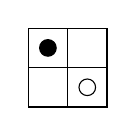
\begin{tikzpicture}[x=1cm]
			\draw (0,0)--(1,0)--(1,1)--(0,1)--cycle;
			\draw (.5,0)--(.5,.5)--(.5,1);
			\draw (0,.5)--(.5,.5)--(1,.5);
			\draw (.75,.25) circle (3pt);
			\filldraw (.25,.75) circle (3pt);
		\end{tikzpicture}
		\caption{$c_{1}$}
	\end{subfigure}%
	%c2
	\begin{subfigure}[t]{.1\textwidth}
		\centering
		
\begin{tikzpicture}[x=1cm]
			\draw (0,0)--(1,0)--(1,1)--(0,1)--cycle;
			\draw (.5,0)--(.5,.5)--(.5,1);
			\draw (0,.5)--(.5,.5)--(1,.5);
			\draw (.25,.25) circle (3pt);
			\filldraw (.25,.75) circle (3pt);
		\end{tikzpicture}
		\caption{$c_{2}$}
	\end{subfigure}%
	%c3
	\begin{subfigure}[t]{.1\textwidth}
		\centering
		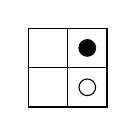
\begin{tikzpicture}[x=1cm]
			\draw (0,0)--(1,0)--(1,1)--(0,1)--cycle;
			\draw (.5,0)--(.5,.5)--(.5,1);
			\draw (0,.5)--(.5,.5)--(1,.5);
			\draw (.75,.25) circle (3pt);
			\filldraw (.75,.75) circle (3pt);
		\end{tikzpicture}
		\caption{$c_{3}$}
	\end{subfigure}%
	%c4
	\begin{subfigure}[t]{.1\textwidth}
		\centering
		
\begin{tikzpicture}[x=1cm]
			\draw (0,0)--(1,0)--(1,1)--(0,1)--cycle;
			\draw (.5,0)--(.5,.5)--(.5,1);
			\draw (0,.5)--(.5,.5)--(1,.5);
			\draw (.25,.25) circle (3pt);
			\filldraw (.75,.75) circle (3pt);
		\end{tikzpicture}
		\caption{$c_{4}$}
	\end{subfigure}%
	%c5
	\begin{subfigure}[t]{.1\textwidth}
		\centering
		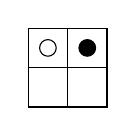
\begin{tikzpicture}[x=1cm]
			\draw (0,0)--(1,0)--(1,1)--(0,1)--cycle;
			\draw (.5,0)--(.5,.5)--(.5,1);
			\draw (0,.5)--(.5,.5)--(1,.5);
			\draw (.25,.75) circle (3pt);
			\filldraw (.75,.75) circle (3pt);
		\end{tikzpicture}
		\caption{$c_{5}$}
	\end{subfigure}%
	%c6
	\begin{subfigure}[t]{.1\textwidth}
		\centering
		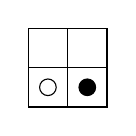
\begin{tikzpicture}[x=1cm]
			\draw (0,0)--(1,0)--(1,1)--(0,1)--cycle;
			\draw (.5,0)--(.5,.5)--(.5,1);
			\draw (0,.5)--(.5,.5)--(1,.5);
			\draw (.25,.25) circle (3pt);
			\filldraw (.75,.25) circle (3pt);
		\end{tikzpicture}
		\caption{$c_{6}$}
	\end{subfigure}
	
	%c7
	\begin{subfigure}[t]{.1\textwidth}
		\centering
		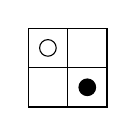
\begin{tikzpicture}[x=1cm]
			\draw (0,0)--(1,0)--(1,1)--(0,1)--cycle;
			\draw (.5,0)--(.5,.5)--(.5,1);
			\draw (0,.5)--(.5,.5)--(1,.5);
			\draw (.25,.75) circle (3pt);
			\filldraw (.75,.25) circle (3pt);
		\end{tikzpicture}
		\caption{$c_{7}$}
	\end{subfigure}%
	%c8
	\begin{subfigure}[t]{.1\textwidth}
		\centering
		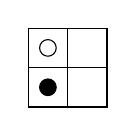
\begin{tikzpicture}[x=1cm]
			\draw (0,0)--(1,0)--(1,1)--(0,1)--cycle;
			\draw (.5,0)--(.5,.5)--(.5,1);
			\draw (0,.5)--(.5,.5)--(1,.5);
			\draw (.25,.75) circle (3pt);
			\filldraw (.25,.25) circle (3pt);
		\end{tikzpicture}
		\caption{$c_{8}$}
	\end{subfigure}%
	%c9
	\begin{subfigure}[t]{.1\textwidth}
		\centering
		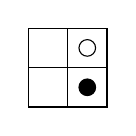
\begin{tikzpicture}[x=1cm]
			\draw (0,0)--(1,0)--(1,1)--(0,1)--cycle;
			\draw (.5,0)--(.5,.5)--(.5,1);
			\draw (0,.5)--(.5,.5)--(1,.5);
			\draw (.75,.75) circle (3pt);
			\filldraw (.75,.25) circle (3pt);
		\end{tikzpicture}
		\caption{$c_{9}$}
	\end{subfigure}%
	%c10
	\begin{subfigure}[t]{.1\textwidth}
		\centering
		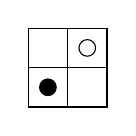
\begin{tikzpicture}[x=1cm]
			\draw (0,0)--(1,0)--(1,1)--(0,1)--cycle;
			\draw (.5,0)--(.5,.5)--(.5,1);
			\draw (0,.5)--(.5,.5)--(1,.5);
			\draw (.75,.75) circle (3pt);
			\filldraw (.25,.25) circle (3pt);
		\end{tikzpicture}
		\caption{$c_{10}$}
	\end{subfigure}%
	%c11
	\begin{subfigure}[t]{.1\textwidth}
		\centering
		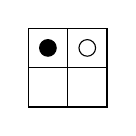
\begin{tikzpicture}[x=1cm]
			\draw (0,0)--(1,0)--(1,1)--(0,1)--cycle;
			\draw (.5,0)--(.5,.5)--(.5,1);
			\draw (0,.5)--(.5,.5)--(1,.5);
			\draw (.75,.75) circle (3pt);
			\filldraw (.25,.75) circle (3pt);
		\end{tikzpicture}
		\caption{$c_{11}$}
	\end{subfigure}%
	%c12
	\begin{subfigure}[t]{.1\textwidth}
		\centering
		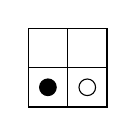
\begin{tikzpicture}[x=1cm]
			\draw (0,0)--(1,0)--(1,1)--(0,1)--cycle;
			\draw (.5,0)--(.5,.5)--(.5,1);
			\draw (0,.5)--(.5,.5)--(1,.5);
			\draw (.75,.25) circle (3pt);
			\filldraw (.25,.25) circle (3pt);
		\end{tikzpicture}
		\caption{$c_{12}$}
	\end{subfigure}
	\caption{Twelve configurations}
\end{figure}

A configuration can be transformed into other configuration according to certain rules. Specifically, we say that the configuration $c_{i}$ can be transformed into the configuration $c_{j}$ $(1 \leq i, j \leq 12, i \neq j)$ if $c_{j}$ can be obtained from $c_{i}$ by performing exactly one of the following two steps:
\begin{enumerate}[{(1)}]
\item moving one of the coins in $c_{i}$ horizontally or vertically to an unoccupied square;
\item interchanging the two coins in $c_{i}$.
\end{enumerate}
Necessarily, if $c_{i}$ can be transformed into $c_{j}$, then $c_{j}$ can be transformed into $c_{i}$. For example, $c_{2}$ can be transformed (i) into $c_{1}$ by shifting the silver coin in $c_{2}$ to the right, (ii) into $c_{4}$ by shifting the gold coin to the right or (iii) into $c_{8}$ by interchanging the two coins (see Figure 1.5).

\begin{figure}[h]
	\centering
	\begin{tikzpicture}[x=2cm, every edge/.style={draw,postaction={decorate,decoration={markings,mark=at position 1.0 with {\arrow[scale=2]{>}}}}}]
		\node[rectangle] (c2) at (1,2) [label=left:$c_{2}:$]{
			\begin{tikzpicture}[x=1cm]
				\draw (0,0)--(1,0)--(1,1)--(0,1)--cycle;
				\draw (.5,0)--(.5,.5)--(.5,1);
				\draw (0,.5)--(.5,.5)--(1,.5);
				\draw (.25,.25) circle (3pt);
				\filldraw (.25,.75) circle (3pt);
			\end{tikzpicture}		
		};
		\node[rectangle] (c1) at (0,0) [label=below:$c_{1}$]{
			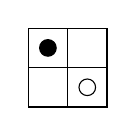
\begin{tikzpicture}[x=1cm]
				\draw (0,0)--(1,0)--(1,1)--(0,1)--cycle;
				\draw (.5,0)--(.5,.5)--(.5,1);
				\draw (0,.5)--(.5,.5)--(1,.5);
				\draw (.75,.25) circle (3pt);
				\filldraw (.25,.75) circle (3pt);
			\end{tikzpicture}
		};
		\node[rectangle] (c4) at (1,0) [label=below:$c_{4}$]{
			
\begin{tikzpicture}[x=1cm]
				\draw (0,0)--(1,0)--(1,1)--(0,1)--cycle;
				\draw (.5,0)--(.5,.5)--(.5,1);
				\draw (0,.5)--(.5,.5)--(1,.5);
				\draw (.25,.25) circle (3pt);
				\filldraw (.75,.75) circle (3pt);
			\end{tikzpicture}
		};
		\node[rectangle] (c8) at (2,0) [label=below:$c_{8}$]{
			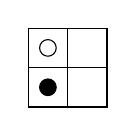
\begin{tikzpicture}[x=1cm]
				\draw (0,0)--(1,0)--(1,1)--(0,1)--cycle;
				\draw (.5,0)--(.5,.5)--(.5,1);
				\draw (0,.5)--(.5,.5)--(1,.5);
				\draw (.25,.75) circle (3pt);
				\filldraw (.25,.25) circle (3pt);
			\end{tikzpicture}
		};
		\path
			(c2) edge (c1)
			(c2) edge (c4)
			(c2) edge (c8)
		;
	\end{tikzpicture}
	\caption{Transformations of the configuration $c_{2}$}
\end{figure}

Now consider the twelve configurations shown in Figure 1.4. Some pairs $c_{i}, c_{j}$ of these configurations, where $1 \leq i, j \leq 12, i \neq j$, can be transformed into each other and some pairs cannot. This situation can also be represented by a graph $F$ where $V(F) = \{c_{1},c_{2},\ldots,c_{12}\}$ and $c_{i}c_{j}$ is an edge of $F$ if $c_{i}$ and $c_{j}$ can be transformed into each other. This graph $F$ is shown in Figure 1.6.
\end{exmp}

\begin{figure}[h]
	\[F:
	\raisebox{-.5\height}
	{
		\begin{tikzpicture}[x=1.5cm, y=1.5cm]
			\foreach \i/\j in {-1/1, -2/2, -3/3, 8/4, 7/5, 6/6, 5/7, 4/8, 3/9, 2/10, 1/11, 0/12} {
				\setcounter{Angle}{90 + \i * 360 / 12};
				\vertex (c\j) at (\theAngle:1) [label=\theAngle:$c_{\j}$]{};
			}
			\path
				(c1) edge (c2)
				(c1) edge (c3)
				(c1) edge (c7)
				(c1) edge (c11)
				(c1) edge (c12)
				(c2) edge (c4)
				(c2) edge (c8)
				(c3) edge (c4)
				(c3) edge (c9)
				(c4) edge (c5)
				(c4) edge (c6)
				(c4) edge (c10)
				(c5) edge (c7)
				(c5) edge (c11)
				(c6) edge (c7)
				(c6) edge (c12)
				(c7) edge (c8)
				(c7) edge (c9)
				(c8) edge (c10)
				(c9) edge (c10)
				(c10) edge (c11)
				(c10) edge (c12)
			;
		\end{tikzpicture}
	}\]
	\caption{Modeling transformations of twelve configurations}
\end{figure}

Let's look at a somewhat related example.

\begin{exmp}
Suppose that we have a collection of 3-letter English words, say
\begin{align*}
ACT, AIM, ARC, ARM, ART, CAR, CAT, OAR, OAT, RAT, TAR.
\end{align*}
We say that a word $W_{1}$ can be transformed into a word $W_{2}$ if $W_{2}$ can be obtained from $W_{1}$ by performing exactly one of the following two steps:
\begin{enumerate}[{(1)}]
\item interchanging two letters of $W_{1}$;
\item replacing a letter in $W_{1}$ by another letter.
\end{enumerate}
Therefore, if $W_{1}$ can be transformed into $W_{2}$, then $W_{2}$ can be transformed into $W_{1}$. This situation can be modeled by a graph $G$, where the given words are the vertices of $G$ and two vertices are adjacent in $G$ if the corresponding words can be transformed into each other. This graph is called \bf{the word graph of the set of words}. For the 11 words above, its word graph $G$ is shown in Figure 1.7.

\begin{figure}[h]
	\[G:
	\raisebox{-.5\height}
	{
		\begin{tikzpicture}[x=1.5cm, y=1.5cm]
			\vertex (AIM) at (0,1.5) [label=above:$AIM$]{};
			\vertex (ARM) at (1,1.5) [label=above:$ARM$]{};
			\vertex (ACT) at (2,0) [label=below:$ACT$]{};
			\vertex (ART) at (2,1) [label=left:$ART$]{};
			\vertex (ARC) at (2,2) [label=above:$ARC$]{};
			\vertex (CAT) at (3,0) [label=below:$CAT$]{};
			\vertex (RAT) at (3,1) [label=above:$RAT$]{};
			\vertex (OAT) at (4,.5) [label=above:$OAT$]{};
			\vertex (OAR) at (5,.5) [label=below:$OAR$]{};
			\vertex (CAR) at (6,0) [label=below:$CAR$]{};
			\vertex (TAR) at (6,1) [label=above:$TAR$]{};
			\path
				(AIM) edge (ARM)
				(ARM) edge (ART)
				(ARM) edge (ARC)
				(ACT) edge (ART)
				(ACT) edge (CAT)
				(ART) edge (ARC)
				(ART) edge (RAT)
				(CAT) edge (RAT)
				(CAT) edge (OAT)
				(CAT) edge (CAR)
				(RAT) edge (OAT)
				(RAT) edge (TAR)
				(OAT) edge (OAR)
				(OAR) edge (CAR)
				(OAR) edge (TAR)
				(CAR) edge (TAR)
			;
		\end{tikzpicture}
	}\]
	\caption{The word graph of a set of 11 words}
\end{figure}

In this case, a graph $G$ is called \bf{a word graph} if $G$ is the word graph of some set $S$ of 3-letter words. For example, the (unlabeled) graph $G$ of Figure 1.8(a) is a word graph because it is the word graph of the set $S = \{BAT, BIT, BUT, BAD, BAR, CAT, HAT\}$, as shown in Figure 1.8(b). (This idea is related to the concept of "isomorphic graphs," which will be discussed in Chapter 3.)
\end{exmp}

\begin{figure}[h]
	\centering
	\begin{subfigure}[b]{.4\textwidth}
		\[G:
		\raisebox{-.5\height}
		{
			\begin{tikzpicture}[x=1.5cm, y=1.5cm]
				\vertex (BAD) at (0,.5){};
				\vertex (BAR) at (.5,0){};
				\vertex (BIT) at (.5,1){};
				\vertex (BAT) at (1,.5){};
				\vertex (HAT) at (1.5,0){};
				\vertex (BUT) at (1.5,1){};
				\vertex (CAT) at (2,.5){};
				\path
					(BAD) edge (BAR)
					(BAD) edge (BAT)
					(BAR) edge (BAT)
					(BIT) edge (BUT)
					(BIT) edge (BAT)
					(BUT) edge (BAT)
					(HAT) edge (BAT)
					(HAT) edge (CAT)
					(CAT) edge (BAT)
				;
			\end{tikzpicture}
		}\]
		\caption{}
	\end{subfigure}%
	\begin{subfigure}[b]{.4\textwidth}
		\[\raisebox{-.5\height}
		{
			\begin{tikzpicture}[x=1.5cm, y=1.5cm]
				\vertex (BAD) at (0,.5) [label=left:$BAD$]{};
				\vertex (BAR) at (.5,0) [label=left:$BAR$]{};
				\vertex (BIT) at (.5,1) [label=left:$BIT$]{};
				\vertex (BAT) at (1,.5) [label=below:$BAT$]{};
				\vertex (HAT) at (1.5,0) [label=right:$HAT$]{};
				\vertex (BUT) at (1.5,1) [label=right:$BUT$]{};
				\vertex (CAT) at (2,.5) [label=right:$CAT$]{};
				\path
					(BAD) edge (BAR)
					(BAD) edge (BAT)
					(BAR) edge (BAT)
					(BIT) edge (BUT)
					(BIT) edge (BAT)
					(BUT) edge (BAT)
					(HAT) edge (BAT)
					(HAT) edge (CAT)
					(CAT) edge (BAT)
				;
			\end{tikzpicture}
		}\]
		\caption{}
	\end{subfigure}
	\caption{A word graph}
\end{figure}

We conclude this section with one last example.

\begin{exmp}
Figure 1.9 shows the traffic lanes at the intersection of two busy streets. When a vehicle approaches this intersection, it could be in one of the nine lanes: L1, L2, \ldots, L9.

\begin{figure}[h]
	\centering
	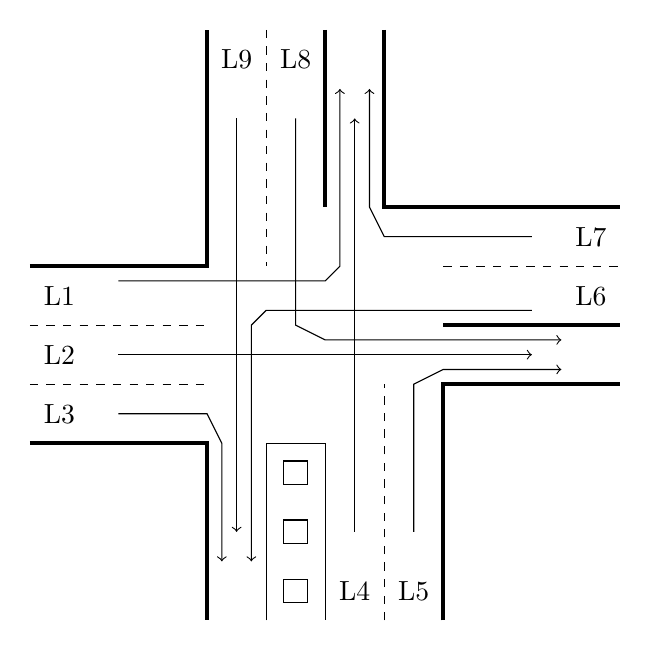
\begin{tikzpicture}[x=1.5cm,y=1.5cm,scale=.5]
		\draw[ultra thick] (0,3)--(3,3)--(3,0);
		\draw[ultra thick] (0,6)--(3,6)--(3,10);
		\draw[ultra thick] (5,10)--(5,7);
		\draw[ultra thick] (6,10)--(6,7)--(10,7);
		\draw[ultra thick] (7,5)--(10,5);
		\draw[ultra thick] (7,0)--(7,4)--(10,4);
		\draw[dashed] (0,4)--(3,4);
		\draw[dashed] (0,5)--(3,5);
		\draw[dashed] (4,10)--(4,6);
		\draw[dashed] (7,6)--(10,6);
		\draw[dashed] (6,0)--(6,4);
		\draw (4,0)--(4,3)--(5,3)--(5,0);
		\draw (4.3,.3)--(4.3,.7)--(4.7,.7)--(4.7,.3)--cycle;
		\draw (4.3,1.3)--(4.3,1.7)--(4.7,1.7)--(4.7,1.3)--cycle;
		\draw (4.3,2.3)--(4.3,2.7)--(4.7,2.7)--(4.7,2.3)--cycle;
		\draw[-{>[scale=2]}] (1.5,3.5)--(3,3.5)--(3.25,3)--(3.25,1);
		\draw[-{>[scale=2]}] (1.5,4.5)--(8.5,4.5);
		\draw[-{>[scale=2]}] (1.5,5.75)--(5,5.75)--(5.25,6)--(5.25,9);
		\draw[-{>[scale=2]}] (3.5,8.5)--(3.5,1.5);
		\draw[-{>[scale=2]}] (4.5,8.5)--(4.5,5)--(5,4.75)--(9,4.75);
		\draw[-{>[scale=2]}] (8.5,6.5)--(6,6.5)--(5.75,7)--(5.75,9);
		\draw[-{>[scale=2]}] (8.5,5.25)--(4,5.25)--(3.75,5)--(3.75,1);
		\draw[-{>[scale=2]}] (6.5,1.5)--(6.5,4)--(7,4.25)--(9,4.25);
		\draw[-{>[scale=2]}] (5.5,1.5)--(5.5,8.5);
		\node at (.5,3.5) {L3};
		\node at (.5,4.5) {L2};
		\node at (.5,5.5) {L1};
		\node at (3.5,9.5) {L9};
		\node at (4.5,9.5) {L8};
		\node at (9.5,6.5) {L7};
		\node at (9.5,5.5) {L6};
		\node at (6.5,.5) {L5};
		\node at (5.5,.5) {L4};
	\end{tikzpicture}
	\caption{Traffic lanes at street intersections}
\end{figure}

This intersection has a traffic light that informs drivers in vehicles in the various lanes when they are permitted to proceed through the intersection. To be sure, there are pairs of lanes containing vehicles that should not enter the intersection at the same time, such as L1 and L7. However, there would be no difficulty for vehicles in L1 and L5 to drive through this intersection at the same time. This situation can be represented by the graph $G$ of Figure 1.10, where $V(G)$ = \{L1,L2,\ldots,L9\} and two vertices (lanes) are joined by an edge if vehicles in these two lanes cannot safely enter the intersection at the same time, as there would be a possibility of an accident.
\end{exmp}

\begin{figure}[h]
	\[G:
	\raisebox{-.5\height}
	{
		\begin{tikzpicture}[x=1.5cm, y=1.5cm]
			\foreach \i/\j in {0/1, -1/2, -2/3, 6/4, 5/5, 4/6, 3/7, 2/8, 1/9} {
				\setcounter{Angle}{90 + \i * 360 / 9};
				\vertex (L\j) at (\theAngle:1) [label=\theAngle:$L\j$]{};
			}
			\path
				(L1) edge (L4)
				(L1) edge (L7)
				(L1) edge (L8)
				(L1) edge (L9)
				(L2) edge (L4)
				(L2) edge (L5)
				(L2) edge (L6)
				(L2) edge (L8)
				(L2) edge (L9)
				(L3) edge (L6)
				(L3) edge (L9)
				(L4) edge (L6)
				(L4) edge (L7)
				(L4) edge (L8)
				(L5) edge (L8)
				(L6) edge (L8)
				(L6) edge (L9)
			;
		\end{tikzpicture}
	}\]
	\caption{The graph $G$ in Example 1.5}
\end{figure}

What we have just seen is how five different situations can be represented by graphs. Actually, in each case, there is a set involved: (1) a set of committees, (2) a set of integers, (3) a set of configurations consisting of two coins on a $2 \times 2$ checkerboard, (4) a set of 3-letter words, (5) a set of traffic lanes at a street intersection. Certain pairs of elements in each set are related in some manner: (1) two committees have a member in common, (2) the sum or difference (in absolute value) of two integers in the set also belongs to the set, (3) two configurations can be transformed into each other according to some rule, (4) two 3-letter words can be transformed into each other by certain movements of letters, (5) cars in certain pairs of traffic lanes cannot enter the intersection at the same time. In each case, a graph $G$ is defined whose vertices are the elements of the set and two vertices of $G$ are adjacent if they are related as described above. The graph $G$ then \it{models} the given situation. Often questions concerning the situations described above arise and can be analyzed by studying the graphs that model them. We will encounter such questions throughout the text and discuss how graphs can be used to help us answer the questions.

\begin{exers}\end{exers}

\begin{exer}
What is a logical question to ask in Example 1.1? Answer this question.
\end{exer}

\begin{exer}
Create an example of your own similar to Example 1.1 with nine editors and eight committees and then draw the corresponding graph.
\end{exer}

\begin{exer}
Let $S = \{2,3,4,7,11,13\}$. Draw the graph $G$ whose vertex set is $S$ and such that $ij \in E(G)$ for $i,j \in S$ if $i+j \in S$ or $|i-j| \in S$.
\end{exer}

\begin{exer}
Let $S = \{-6,-3,0,3,6\}$. Draw the graph $G$ whose vertex set is $S$ and such that $ij \in E(G)$ for $i,j \in S$ if $i+j \in S$ or $|i-j| \in S$.
\end{exer}

\begin{exer}
Create your own set $S$ of integers and draw the graph $G$ whose vertex set is $S$ and such that $ij \in E(G)$ if $i$ and $j$ are related by some rule imposed on $i$ and $j$.
\end{exer}

\begin{exer}
Consider the twelve configurations $c_{1},c_{2},\ldots,c_{12}$ in Figure 1.4. For every two configurations $c_{i}$ and $c_{j}$, where $1 \leq i,j \leq 12, i \neq j$, it may be possible to obtain $c_{j}$ from $c_{i}$ by first shifting one of the coins in $c_{i}$ horizontally or vertically \it{and} then interchanging the two coins. Model this by a graph $F$ such that $V(F) = \{c_{1},c_{2},\ldots,c_{12}\}$ and $c_{i}c_{j}$ is an edge of $F$ if $c_{i}$ and $c_{j}$ can be transformed into each other by this 2-step process.
\end{exer}

\begin{exer}
Following Example 1.4,
\begin{enumerate}[{(a)}]
\item give an example of ten 3-letter words, none of which are mentioned in Example 1.4 and whose corresponding word graph has at least six edges. Draw this graph.
\item give a set of five 3-letter words whose word graph is shown in Figure 1.11 (with the vertices appropriately labeled).
\begin{figure}[h]
	\centering
	\begin{tikzpicture}[x=1.5cm, y=1.5cm]
		\foreach \i in {1,2,3,4,5} {
			\vertex (\i) at (\i,0){};
		}
		\path
			(1) edge (2)
			(2) edge (3)
			(3) edge (4)
			(4) edge (5)
		;
	\end{tikzpicture}
	\caption{The graph in Exercise 1.7(b)}
\end{figure}
\item give a set of five 3-letter words whose word graph is shown in Figure 1.12 (with the vertices appropriately labeled).
\begin{figure}[h]
	\centering
	\begin{tikzpicture}[x=1.5cm, y=1.5cm]
		\foreach \i in {1,2,3,4,5} {
			\setcounter{Angle}{90 + \i * 360 / 5};
			\vertex (\i) at (\theAngle:.75){};
		}
		\path
			(1) edge (2)
			(1) edge (5)
			(2) edge (3)
			(3) edge (4)
			(4) edge (5)
		;
	\end{tikzpicture}
	\caption{The graph in Exercise 1.7(c)}
\end{figure}
\end{enumerate}
\end{exer}

\begin{exer}
Let $S$ be a finite set of 3-letter and/or 4-letter words. In this case, the word graph $G(S)$ of $S$ is that graph whose vertex set is $S$ and such that two vertices (words) $w_{1}$ and $w_{2}$ are adjacent if either (1) or (2) below occurs:
\begin{enumerate}[{(1)}]
\item one of the words can be obtained from the other by replacing one letter by another letter,
\item $w_{1}$ is a 3-letter word and $w_{2}$ is a 4-letter word and $w_{2}$ can be obtained from $w_{1}$ by the insertion of a single letter (anywhere, including the beginning or the end) into $w_{1}$.
\end{enumerate}
\begin{enumerate}[{(a)}]
\item Find six sets $S_{1},S_{2},\ldots,S_{6}$ of 3-letter and/or 4-letter words so that for each integer $i$ $(1 \leq i \leq 6)$ the graph $G_{i}$ of Figure 1.13 is the word graph of $S_{i}$.
\item For another graph $H$ (of your choice), determine whether $H$ is a word graph of some set.
\end{enumerate}

\begin{figure}[h]
	\centering
	\captionsetup[subfigure]{labelformat=empty}
	\begin{subfigure}[b]{.1\textwidth}
		\centering
		\begin{tikzpicture}[x=1.5cm]
			\foreach \i in {0,1,2,3} {
				\vertex (\i) at (0,\i * .5){};
			}
			\path
				(0) edge (1)
				(1) edge (2)
				(2) edge (3)
			;
		\end{tikzpicture}
		\caption{$G_{1}$}
	\end{subfigure}%
	\begin{subfigure}[b]{.1\textwidth}
		\centering
		\begin{tikzpicture}[x=1.5cm]
			\foreach \i in {0,1,2} {
				\setcounter{Angle}{270 + \i * 360 / 3};
				\vertex (\i) at (\theAngle:.5){};
			}
			\vertex (3) at (0,0){};
			\path
				(3) edge (0)
				(3) edge (1)
				(3) edge (2)
			;
		\end{tikzpicture}
		\caption{$G_{2}$}
	\end{subfigure}%
	\begin{subfigure}[b]{.1\textwidth}
		\centering
		\begin{tikzpicture}[x=1.5cm]
			\foreach \i in {0,1,2} {
				\setcounter{Angle}{270 + \i * 360 / 3};
				\vertex (\i) at (\theAngle:.5){};
			}
			\vertex (3) at (0,0){};
			\path
				(3) edge (0)
				(3) edge (1)
				(3) edge (2)
				(1) edge (2)
			;
		\end{tikzpicture}
		\caption{$G_{3}$}
	\end{subfigure}%
	\begin{subfigure}[b]{.1\textwidth}
		\centering
		\begin{tikzpicture}[x=1.5cm]
			\foreach \i in {0,1,2,3} {
				\setcounter{Angle}{45 + \i * 360 / 4};
				\vertex (\i) at (\theAngle:.5){};
			}
			\path
				(0) edge (1)
				(0) edge (3)
				(1) edge (2)
				(2) edge (3)
			;
		\end{tikzpicture}
		\caption{$G_{4}$}
	\end{subfigure}%
	\begin{subfigure}[b]{.1\textwidth}
		\centering
		\begin{tikzpicture}[x=1.5cm]
			\foreach \i in {0,1,2,3} {
				\setcounter{Angle}{45 + \i * 360 / 4};
				\vertex (\i) at (\theAngle:.5){};
			}
			\path
				(0) edge (1)
				(0) edge (3)
				(1) edge (2)
				(1) edge (3)
				(2) edge (3)
			;
		\end{tikzpicture}
		\caption{$G_{5}$}
	\end{subfigure}%
	\begin{subfigure}[b]{.1\textwidth}
		\centering
		\begin{tikzpicture}[x=1.5cm]
			\foreach \i in {0,1,2,3} {
				\setcounter{Angle}{45 + \i * 360 / 4};
				\vertex (\i) at (\theAngle:.5){};
			}
			\path
				(0) edge (1)
				(0) edge (2)
				(0) edge (3)
				(1) edge (2)
				(1) edge (3)
				(2) edge (3)
			;
		\end{tikzpicture}
		\caption{$G_{6}$}
	\end{subfigure}
	\caption{The graphs for Exercise 1.8(a)}
\end{figure}
\end{exer}

\begin{exer}
Define a word graph differently from the word graphs defined in Example 1.4 and Exercise 1.8 and illustrate your definition.
\end{exer}

\begin{exer}
\begin{figure}[h]
	\centering
	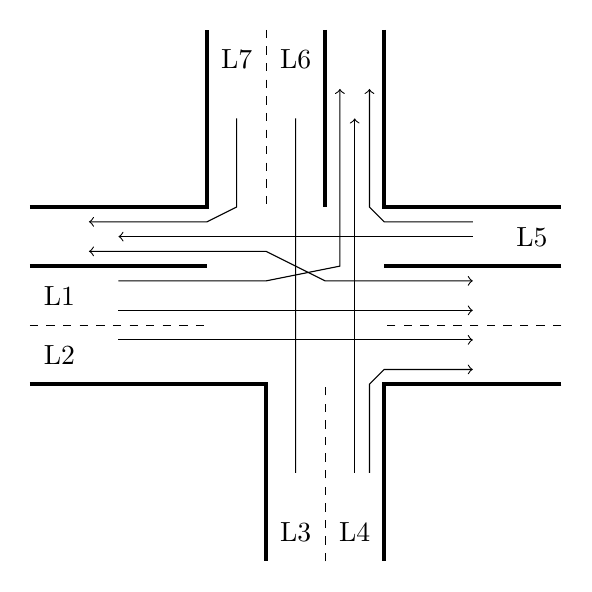
\begin{tikzpicture}[x=1.5cm,y=1.5cm,scale=.5]
		\draw[ultra thick] (0,3)--(4,3)--(4,0);
		\draw[ultra thick] (0,5)--(3,5);
		\draw[ultra thick] (0,6)--(3,6)--(3,9);
		\draw[ultra thick] (5,9)--(5,6);
		\draw[ultra thick] (6,9)--(6,6)--(9,6);
		\draw[ultra thick] (9,5)--(6,5);
		\draw[ultra thick] (9,3)--(6,3)--(6,0);
		\draw[dashed] (0,4)--(3,4);
		\draw[dashed] (4,9)--(4,6);
		\draw[dashed] (9,4)--(6,4);
		\draw[dashed] (5,0)--(5,3);
		\draw[-{>[scale=2]}] (1.5,3.75)--(7.5,3.75);
		\draw[-{>[scale=2]}] (1.5,4.25)--(7.5,4.25);
		\draw[-{>[scale=2]}] (1.5,4.75)--(4,4.75)--(5.25,5)--(5.25,8);
		\draw[-{>[scale=2]}] (3.5,7.5)--(3.5,6)--(3,5.75)--(1,5.75);
		\draw[-{>[scale=2]}] (4.5,7.5)--(4.5,5)--(5,4.75)--(7.5,4.75);
		\draw[-{>[scale=2]}] (7.5,5.75)--(6,5.75)--(5.75,6)--(5.75,8);
		\draw[-{>[scale=2]}] (7.5,5.5)--(1.5,5.5);
		\draw[-{>[scale=2]}] (5.75,1.5)--(5.75,3)--(6,3.25)--(7.5,3.25);
		\draw[-{>[scale=2]}] (5.5,1.5)--(5.5,7.5);
		\draw[-{>[scale=2]}] (4.5,1.5)--(4.5,5)--(4,5.25)--(1,5.25);
		\node at (.5,3.5) {L2};
		\node at (.5,4.5) {L1};
		\node at (3.5,8.5) {L7};
		\node at (4.5,8.5) {L6};
		\node at (8.5,5.5) {L5};
		\node at (5.5,.5) {L4};
		\node at (4.5,.5) {L3};
	\end{tikzpicture}
	\caption{Traffic lanes at a street intersection in Exercise 1.10}
\end{figure}

Figure 1.14 illustrates the traffic lanes at the intersection of two streets. When a vehicle approaches this intersection, it could be in one of the seven lanes: L1, L2, \ldots, L7. Draw a graph $G$ that models this situation, where $V(G)$ = \{L1,L2,\ldots,L7\} and wher two vertices are joined by an edge if vehicles in these two lanes cannot safely enter this intersection at the same time.
\end{exer}
\section{Connected Graphs}
In order to analyze certain situations that can be modeled by graphs, we must have a better understanding of graphs. As with all areas of mathematics, there is a certain amount of terminology with which we must first be familiar in order to discuss graphs and their properties. Becoming aware of this fundamental terminology is our current goal. First, let's review some concepts and introduce others. Recall that a graph $G$ consists of a finite nonempty set $V$ of vertices and a set $E$ of 2-element subsets of $V$ called edges. If $e = uv$ is an edge of $G$, then the adjacent vertices $u$ and $v$ are said to be \bf{joined} by the edge $e$. The vertices $u$ and $v$ are referred to as \bf{neighbors} of each other. In this case, the vertex $u$ and the edge $e$ (as well as $v$ and $e$) are said to be \bf{incident} with each other. Distinct edges incident with a common vertex are \bf{adjacent edges}.

As we mentioned earlier, although graphs are defined in terms of sets, it is customary and convenient to represent graphs by (and, in fact, to consider them as) diagrams. A graph $G$ with vertex set $V = \{u,v,w,x,y\}$ and edge set $E = \{uv,vw,vx,vy,wy,xy\}$ is shown in Figure 1.15. Since this graph has five vertices and six edges, its order is 5 and its size is 6. In this graph $G$, the vertices $u$ and $v$ are adjacent, while $u$ and $w$ are not adjacent. The vertex $v$ is incident the edge $vw$ but not with the edge $wy$. The edges $uv$ and $vw$ are adjacent, but $uv$ and $xy$ are not adjacent.

\begin{figure}[h]
	\centering
	%G
	\begin{subfigure}[b]{.3\textwidth}
		\centering
		\[G:
		\raisebox{-.5\height}
		{
			\begin{tikzpicture}[scale=.75]
				\vertex (u) at (90:3) [label=right:$u$]{};
				\vertex (v) at (90:1.5) [label=right:$v$]{};
				\vertex (w) at (180:1) [label=left:$w$]{};
				\vertex (x) at (0:1) [label=right:$x$]{};
				\vertex (y) at (270:1.5) [label=below:$y$]{};
				\path
					(u) edge (v)
					(v) edge (w)
					(v) edge (x)
					(v) edge node[right]{$e$} (y)
					(w) edge (y)
					(x) edge node[pos=.4,right]{$e'$} (y)
				;
			\end{tikzpicture}
		}\]
	\end{subfigure}%
	%H
	\begin{subfigure}[b]{.3\textwidth}
		\centering
		\[H:
		\raisebox{-.5\height}
		{
			\begin{tikzpicture}[scale=.75]
				\vertex (v) at (90:1.5) [label=right:$v$]{};
				\vertex (w) at (180:1) [label=left:$w$]{};
				\vertex (x) at (0:1) [label=right:$x$]{};
				\vertex (y) at (270:1.5) [label=below:$y$]{};
				\path
					(v) edge (w)
					(w) edge (y)
					(x) edge (y)
				;
			\end{tikzpicture}
		}\]
	\end{subfigure}%
	%F
	\begin{subfigure}[b]{.3\textwidth}
		\centering
		\[F:
		\raisebox{-.5\height}
		{
			\begin{tikzpicture}[scale=.75]
				\vertex (v) at (90:1.5) [label=right:$v$]{};
				\vertex (w) at (180:1) [label=left:$w$]{};
				\vertex (x) at (0:1) [label=right:$x$]{};
				\path
					(v) edge (w)
					(v) edge (x)
				;
			\end{tikzpicture}
		}\]
	\end{subfigure}
	
	%F'
	\begin{subfigure}[b]{.4\textwidth}
		\centering
		\[F':
		\raisebox{-.5\height}
		{
			\begin{tikzpicture}[scale=.75]
				\vertex (v) at (90:1.5) [label=right:$v$]{};
				\vertex (x) at (0:1) [label=right:$x$]{};
				\vertex (y) at (270:1.5) [label=below:$y$]{};
				\path
					(v) edge node[right]{$e$} (y)
					(x) edge node[pos=.4,right]{$e'$} (y)
				;
			\end{tikzpicture}
		}\]
	\end{subfigure}%
	%G-e
	\begin{subfigure}[b]{.4\textwidth}
		\centering
		\[G-e:
		\raisebox{-.5\height}
		{
			\begin{tikzpicture}[scale=.75]
				\vertex (u) at (90:3) [label=right:$u$]{};
				\vertex (v) at (90:1.5) [label=right:$v$]{};
				\vertex (w) at (180:1) [label=left:$w$]{};
				\vertex (x) at (0:1) [label=right:$x$]{};
				\vertex (y) at (270:1.5) [label=below:$y$]{};
				\path
					(u) edge (v)
					(v) edge (w)
					(v) edge (x)
					(w) edge (y)
					(x) edge (y)
				;
			\end{tikzpicture}
		}\]
	\end{subfigure}
	\caption{A graph $G$ and some of its subgraphs}
\end{figure}

A graph $H$ is called a \bf{subgraph} of a graph $G$, written $H \subseteq G$, if $V(H) \subseteq V(G)$ and $E(H) \subseteq E(G)$. We also say that $G$ contains $H$ as a subgraph. If $H \subseteq G$ and either $V(H)$ is a proper subset of $V(G)$ or $E(H)$ is a proper subset of $E(G)$, then $H$ is a \bf{proper subgraph} of $G$. So the graph $H$ of Figure 1.15 is a subgraph of the graph $G$ shown in that figure; indeed, $H$ is a proper subgraph of $G$. If a subgraph of a graph $G$ has the same vertex set as $G$, then it is a \bf{spanning subgraph} of $G$.

A subgraph $F$ of a graph $G$ is called an \bf{induced subgraph} of $G$ if whenever $u$ and $v$ are vertices of $F$ and $uv$ is an edge of $G$, then $uv$ is an edge of $F$ as well. Therefore, the graph $H$ of Figure 1.15 is not an induced subgraph of the graph $G$ of Figure 1.15 since, for example, $v,x \in V(H)$ and $vx \in E(G)$ but $vx \centernot\in E(H)$. On the other hand, the graph $F$ of Figure 1.15 is an induced subgraph of $G$. If $S$ is a nonempty set of vertices of a graph $G$, then the \bf{subgraph of} $G$ \bf{induced by} $S$ is the induced subgraph with vertex set $S$. This induced subgraph is denoted by $G[S]$. For a nonempty set $X$ of edges, the \bf{subgraph} $G[X]$ \bf{induced by} $X$ has edge set $X$ and consists of all vertices that are incident with at least one edge in $X$. This subgraph is called an \bf{edge-induced subgraph} of $G$. Sometimes $\langle S \rangle_{G}$ and $\langle X \rangle_{G}$ are used for $G[S]$ and $G[X]$, respectively. The graph $F'$ of Figure 1.15 is an edge-induced subgraph of $G$ in that figure; indeed, $F' = G[X']$, where $X' = \{e,e'\}$.

Any proper subgraph of a graph $G$ can be obtained by removing vertices and edges from $G$. For an edge $e$ of $G$, we write $G-e$ for the spanning subgraph of $G$ whose edge set consists of all edges of $G$ except $e$. More generally, if $X$ is a set of edges of $G$, then $G-X$ is the spanning subgraph of $G$ with $E(G-X) = E(G) \smallsetminus X$. For the graph $G$ of Figure 1.15 and $e = vy$, the subgraph $G - e$ is shown. If $X = \{e_{1},e_{2},\ldots,e_{k}\}$, then we also write $G-X$ as $G-e_{1}-e_{2}-\cdots-e_{k}$.

For a vertex $v$ of a nontrivial graph $G$, the subgraph $G-v$ consists of all vertices of $G$ except $v$ and all edges of $G$ except those incident with $v$. For a proper subset $U$ of $V(G)$, the subgraph $G-U$ has vertex set $V(G) \smallsetminus U$ and its edge set consists of all edges of $G$ joining two vertices in $V(G) \smallsetminus U$. Necessarily, $G-U$ is an induced subgraph of $G$. For $U = \{u,y\}$ in the graph $G$ of Figure 1.15, $G-U$ is the subgraph $F$ shown in that figure.

If $u$ and $v$ are nonadjacent vertices of a graph $G$, then $e = uv \centernot\in E(G)$. By $G+e$, we mean the graph with vertex set $V(G)$ and edge set $E(G) \union \{e\}$. Thus $G$ is a spanning subgraph of $G+e$.

Many of the concepts that occur in graph theory and which we will investigate in detail later concern various ways in which one can "move about" in a graph. In particular, if we think of the vertices of a graph as locations and the edges as roads between certain pairs of locations, then the graph can be considered as modeling some community. There is a variety of kinds of trips that can be taken in the community.

Let's start at some vertex $u$ of a graph $G$. If we proceed from $u$ to a neighbor of $u$ and then to a neighbor of that vertex and so on, until we finally come to a stop at a vertex $v$, then we have just described a walk from $u$ to $v$ in $G$. More formally, a $u-v$ \bf{walk} $W$ in $G$ is a sequence of vertices in $G$, beginning with $u$ and ending at $v$ such that consecutive vertices in the sequence are adjacent, that is, we can express $W$ as
\begin{equation}
W = (u=v_{0},v_{1},\ldots,v_{k}=v),
\end{equation}
where $k \geq 0$ and $v_{i}$ and $v_{i+1}$ are adjacent for $i = 0,1,2,\ldots,k-1$. Each vertex $v_{i}$ $(0 \leq i \leq k)$ and each edge $v_{i}v_{i+1}$ $(0 \leq i \leq k-1)$ is said to lie on or belong to $W$. Notice that the definition of the walk $W$ does not require the listed vertices to be distinct; in fact, even $u$ and $v$ are not required to be distinct. However, every two consecutive vertices in $W$ are distinct since they are adjacent. If $u=v$, then the walk $W$ is \bf{closed}; while if $u \neq v$, then $W$ is \bf{open}. As we move from one vertex of $W$ to the next, we are actually encountering or traversing edges of $G$, possibly traversing some edges of $G$ more than once. The number of edges encountered in a walk (including multiple occurrences of an edge) is called the \bf{length} of the walk. Thus the length of the walk $W$ defined in (1.1) is $k$.

For the graph $G$ of Figure 1.16,
\begin{equation}
W = (x,y,w,y,v,w)
\end{equation}
is therefore a walk, indeed an $x-w$ walk of length 5 (one less than the number of occurrences of vertices in the walk). A walk of length 0 is a \bf{trivial walk}. So $W = (v)$ is a trivial walk. (By this definition, those people who feel guilty about not exercising need not feel guilty any longer as going for a daily "walk" just became easier.)

Provided we continue to proceed from a vertex to one of its neighbors (and eventually stop), there is essentially no conditions on a walk. However, there will be occasions when we want to place restrictions on certain types of walks.

\begin{figure}[h]
	\[G:
	\raisebox{-.5\height}
	{
		\begin{tikzpicture}[x=1.5cm,y=1.5cm]
			\foreach \i/\j in {1/u, 0/v, 2/x, 3/y} {
				\setcounter{Angle}{45 + \i * 360 / 4};
				\vertex (\j) at (\theAngle:1) [label=\theAngle:$\j$]{};
			}
			\vertex (w) at (0,0) [label=above:$w$]{};
			\path
				(u) edge (v)
				(u) edge (w)
				(v) edge (w)
				(v) edge (y)
				(w) edge (x)
				(w) edge (y)
				(x) edge (y)
			;
		\end{tikzpicture}
	}\]
	\caption{Illustrating walks in a graph}
\end{figure}

Borrowing terminology from the Old West, we define a $u-v$ \bf{trail} in a graph $G$ to be a $u-v$ walk in which no edge is traversed more than once. Thus, the $x-w$ walk $W$ in (1.2) is \it{not} an $x-w$ trail as the edge $wy$ is repeated. On the other hand,
\begin{equation}
T = (u,w,y,x,w,v)
\end{equation}
is a $u-v$ trail in the graph $G$ of Figure 1.16. Notice that this trail $T$ repeats the vertex $w$. This is perfectly permissible. Although the definition of a trail stipulates that no edge can be repeated, no such condition is placed on vertices.

A $u-v$ walk in a graph in which no vertices are repeated is a $u-v$ \bf{path}. While the $u-v$ trail $T$ in (1.3) is not a $u-v$ path in the graph $G$ of Figure 1.16 (since the vertex $w$ is repeated),
\begin{align*}
P = (u,w,y,v)
\end{align*}
\it{is} a $u-v$ path. If no vertex in a walk is repeated (thereby producing a path), then no edge is repeated either. Hence every path is a trail.

If a $u-v$ walk in a graph is followed by a $v-w$ walk, then a $u-w$ walk results. In particular, a $u-v$ path followed by a $v-w$ path is a $u-w$ walk $W$ but not necessarily a $u-w$ path, as vertices in $W$ may be repeated. While not every walk is a path, if a graph contains a $u-v$ walk, then it must also contain a $u-v$ path. This is our first theorem.

\begin{thm}
If a graph $G$ contains a $u-v$ walk of length $l$, then $G$ contains a $u-v$ path of length at most $l$.
\end{thm}

\begin{pf}
Among all $u-v$ walks in $G$, let
\begin{align*}
P = (u = u_{0},u_{1},\ldots,u_{k} = v)
\end{align*}
be a $u-v$ walk of smallest length $k$. Therefore, $k \leq l$. We claim that $P$ is a $u-v$ path. Assume, to the contrary, that this is not the case. Then some vertex of $G$ must be repeated in $P$, say $u_{i} = u_{j}$ for some $i$ and $j$ with $0 \leq i < j \leq k$. If we then delete the vertices $u_{i+1},u_{i+2},\ldots,u_{j}$ from $P$, we arrive at the $u-v$ walk
\begin{align*}
(u = u_{0},u_{1},\ldots,u_{i-1},u_{i} = u_{j},u_{j+1},\ldots,u_{k} = v)
\end{align*}
whose length is less than $k$, which is impossible. Therefore, as claimed, $P$ is a $u-v$ path of length $k \leq l$.
\end{pf}

A \bf{circuit} in a graph $G$ is a closed trail of length 3 or more. Hence a circuit begins and ends at the same vertex but repeats no edges. A circuit can be described by choosing any of its vertices as the beginning (and ending) vertex provided the vertices are listed in the same cyclic order. In a circuit, vertices can be repeated, in addition to the first and last. For example, in the graph $G$ of Figure 1.16,
\begin{equation}
C = (y,w,u,v,w,x,y) \text{ or } C = (x,y,w,u,v,w,x) \text{ or } C = (w,x,y,w,u,v,w)
\end{equation}
is a circuit. A circuit that repeats no vertex, except for the first and last, is a \bf{cycle}. A $k$\bf{-cycle} is a cycle of length $k$. A 3-cycle is also referred to as a \bf{triangle}. A cycle of odd length is called an \bf{odd cycle}; while, not surprisingly, a cycle of even length is called an \bf{even cycle}. In the graph $G$ of Figure 1.16, the circuit $C$ in (1.4) is not a cycle, while
\begin{align*}
C' = (x,y,v,w,x)
\end{align*}
\it{is} a cycle, namely a 4-cycle. If a vertex of a cycle is deleted, then a path is obtained. This is not necessarily true for circuits, however.

The vertices and edges of a trail, path, circuit or cycle in a graph $G$ form a subgraph of $G$, also called a \bf{trail}, \bf{path}, \bf{circuit} or \bf{cycle}. Hence a path, for example, is used to describe both a manner of traversing certain vertices and edges of $G$ and a subgraph consisting of those vertices and edges. The graph $G$ of Figure 1.16 is shown again in Figure 1.17. Thus the subgraphs $G_{1}, G_{2}, G_{3}, G_{4}$ of the graph $G$ are a trail, path, circuit and cycle, respectively.

\begin{figure}[h]
	\centering
	%G
	\begin{subfigure}[b]{.3\textwidth}
		\[G:
		\raisebox{-.5\height}
		{
			\begin{tikzpicture}[x=1.5cm,y=1.5cm]
				\foreach \i/\j in {1/u, 0/v, 2/x, 3/y} {
					\setcounter{Angle}{45 + \i * 360 / 4};
					\vertex (\j) at (\theAngle:1) [label=\theAngle:$\j$]{};
				}
				\vertex (w) at (0,0) [label=above:$w$]{};
				\path
					(u) edge (v)
					(u) edge (w)
					(v) edge (w)
					(v) edge (y)
					(w) edge (x)
					(w) edge (y)
					(x) edge (y)
				;
			\end{tikzpicture}
		}\]
	\end{subfigure}%
	%G1
	\begin{subfigure}[b]{.3\textwidth}
		\[G_{1}:
		\raisebox{-.5\height}
		{
			\begin{tikzpicture}[x=1.5cm,y=1.5cm]
				\foreach \i/\j in {1/u, 0/v, 2/x, 3/y} {
					\setcounter{Angle}{45 + \i * 360 / 4};
					\vertex (\j) at (\theAngle:1) [label=\theAngle:$\j$]{};
				}
				\vertex (w) at (0,0) [label=above:$w$]{};
				\path
					(u) edge (w)
					(v) edge (w)
					(w) edge (x)
					(w) edge (y)
					(x) edge (y)
				;
			\end{tikzpicture}
		}\]
	\end{subfigure}%
	%G2
	\begin{subfigure}[b]{.3\textwidth}
		\[G_{2}:
		\raisebox{-.5\height}
		{
			\begin{tikzpicture}[x=1.5cm,y=1.5cm]
				\foreach \i/\j in {1/u, 0/v, 3/y} {
					\setcounter{Angle}{45 + \i * 360 / 4};
					\vertex (\j) at (\theAngle:1) [label=\theAngle:$\j$]{};
				}
				\vertex (w) at (0,0) [label=above:$w$]{};
				\path
					(u) edge (w)
					(v) edge (y)
					(w) edge (y)
				;
			\end{tikzpicture}
		}\]
	\end{subfigure}
	
	%G3
	\begin{subfigure}[b]{.4\textwidth}
		\[G_{3}:
		\raisebox{-.5\height}
		{
			\begin{tikzpicture}[x=1.5cm,y=1.5cm]
				\foreach \i/\j in {1/u, 0/v, 2/x, 3/y} {
					\setcounter{Angle}{45 + \i * 360 / 4};
					\vertex (\j) at (\theAngle:1) [label=\theAngle:$\j$]{};
				}
				\vertex (w) at (0,0) [label=above:$w$]{};
				\path
					(u) edge (v)
					(u) edge (w)
					(v) edge (w)
					(w) edge (x)
					(w) edge (y)
					(x) edge (y)
				;
			\end{tikzpicture}
		}\]
	\end{subfigure}%
	%G4
	\begin{subfigure}[b]{.4\textwidth}
		\[G_{4}:
		\raisebox{-.5\height}
		{
			\begin{tikzpicture}[x=1.5cm,y=1.5cm]
				\foreach \i/\j in {0/v, 2/x, 3/y} {
					\setcounter{Angle}{45 + \i * 360 / 4};
					\vertex (\j) at (\theAngle:1) [label=\theAngle:$\j$]{};
				}
				\vertex (w) at (0,0) [label=above:$w$]{};
				\path
					(v) edge (w)
					(v) edge (y)
					(w) edge (x)
					(x) edge (y)
				;
			\end{tikzpicture}
		}\]
	\end{subfigure}
	\caption{Trails, paths, circuits and cycles as subgraphs of a graph}
\end{figure}

We will have a special interest in graphs $G$ in which it is possible to travel from each vertex of $G$ to any other vertex of $G$. If $G$ contains a $u-v$ path, then $u$ and $v$ are said to be \bf{connected} and $u$ \bf{is connected to} $v$ (and $v$ is connected to $u$). So, saying that $u$ and $v$ are connected only means that there is some $u-v$ path in $G$; it doesn't say that $u$ and $v$ are joined by an edge. Of course, if $u$ \it{is} joined to $v$, then $u$ is connected to $v$ as well. A graph $G$ is \bf{connected} if every two vertices of $G$ are connected, that is, if $G$ contains a $u-v$ path for every pair $u,v$ of vertices of $G$. By Theorem 1.6, G is connected if and only if G contains a $u-v$ walk for every pair $u,v$ of vertices of $G$. Since every vertex is connected to itself, the trivial graph is connected.

A graph $G$ that is not connected is \bf{disconnected}. A connected subgraph of $G$ that is not a proper subgraph of any other connected subgraph of $G$ is a \bf{component} of $G$. The number of components of a graph $G$ is denoted by $k(G)$. Thus a graph $G$ is connected if and only if $k(G) = 1$. While the graph $G$ of Figure 1.16 is connected, the graph $H$ of Figure 1.18 is disconnected since, for example, there is no $s-w$ path in $H$. There is no $x-z$ path either. The graph $H$ has three components, namely $H_{1}$, $H_{2}$ and $H_{3}$ and so $k(H) = 3$.

For subgraphs $G_{1},G_{2},\ldots,G_{k}$, $k \geq 2$, of a graph $G$, with mutually disjoint vertex sets, we write $G = G_{1} \union G_{2} \union \ldots \union G_{k}$ if every vertex and every edge of $G$ belong to exactly one of these subgraphs. In this case, $G$ is the \bf{union} of the graphs $G_{1},G_{2},\ldots,G_{k}$. In particular, we write $G = G_{1} \union G_{2} \union \ldots \union G_{k}$ if $G_{1},G_{2},\ldots,G_{k}$ are components of $G$. That is, every graph is the union of its components. Therefore, we can write $H = H_{1} \union H_{2} \union H_{3}$ for the graphs in Figure 1.18.

\begin{figure}[h]
	\centering
	%H=H1 U H2 U H3
	\begin{subfigure}[b]{.9\textwidth}
		\[H = H_{1} \union H_{2} \union H_{3}:
		\raisebox{-.5\height}
		{
			\begin{tikzpicture}
				\vertex (s) at (0,1) [label=left:$s$]{};
				\vertex (t) at (1,1) [label=right:$t$]{};
				\vertex (u) at (0,0) [label=left:$u$]{};
				\vertex (v) at (1,0) [label=right:$v$]{};
				\vertex (w) at (2,1) [label=below:$w$]{};
				\vertex (x) at (3,1) [label=below:$x$]{};
				\vertex (y) at (4,1) [label=below:$y$]{};
				\vertex (z) at (5,1) [label=below:$z$]{};
				\path
					(s) edge (t)
					(s) edge (u)
					(t) edge (v)
					(u) edge (v)
					(w) edge (x)
					(x) edge (y)
				;
			\end{tikzpicture}
		}\]
	\end{subfigure}
	
	%H1
	\begin{subfigure}[b]{.3\textwidth}
		\[H_{1}:
		\raisebox{-.5\height}
		{
			\begin{tikzpicture}
				\vertex (s) at (0,1) [label=left:$s$]{};
				\vertex (t) at (1,1) [label=right:$t$]{};
				\vertex (u) at (0,0) [label=left:$u$]{};
				\vertex (v) at (1,0) [label=right:$v$]{};
				\path
					(s) edge (t)
					(s) edge (u)
					(t) edge (v)
					(u) edge (v)
				;
			\end{tikzpicture}
		}\]
	\end{subfigure}%
	%H2
	\begin{subfigure}[b]{.3\textwidth}
		\[H_{2}:
		\raisebox{-.5\height}
		{
			\begin{tikzpicture}
				\vertex (w) at (0,1) [label=below:$w$]{};
				\vertex (x) at (1,1) [label=below:$x$]{};
				\vertex (y) at (2,1) [label=below:$y$]{};
				\path
					(w) edge (x)
					(x) edge (y)
				;
			\end{tikzpicture}
		}\]
	\end{subfigure}%
	%H3
	\begin{subfigure}[b]{.3\textwidth}
		\[H_{3}:
		\raisebox{-.5\height}
		{
			\begin{tikzpicture}
				\vertex (z) at (0,1) [label=below:$z$]{};
			\end{tikzpicture}
		}\]
	\end{subfigure}
	\caption{A disconnected graph and its components}
\end{figure}

Components can also be defined by means of an equivalence relation. (Equivalence relations are reviewed in Appendix B.1.)

\begin{thm}
Let $R$ be the relation defined on the vertex set of a graph $G$ by $u R v$, where $u,v \in V(G)$, if $u$ is connected to $v$, that is if $G$ contains a $u-v$ path. Then $R$ is an equivalence relation.
\end{thm}

\begin{pf}
It is immediate that $R$ is reflexive and symmetric. It remains therefore only to show that $R$ is transitive. Let $u,v,w \in V(G)$ such that $u R v$ and $v R w$. Hence $G$ contains a $u-v$ path $P'$ and a $v-w$ path $P''$. As we have seen earlier, following $P'$ by $P''$ produces a $u-w$ walk $W$. By Theorem 1.6, $G$ contains a $u-w$ path and so $u R w$.
\end{pf}

The equivalence relation described in Theorem 1.7 produces a partition of the vertex set of every graph $G$ into equivalence classes. The subgraph of $G$ induced by the vertices in an equivalence class is a component of $G$. Exercise 1.14 asks you to show this. As a consequence, we have the following:
\begin{cons}
Each vertex and each edge of a graph $G$ belong to exactly one component of $G$. This implies that if $G$ is a disconnected graph and $u$ and $v$ are vertices belonging to different components of $G$, then $uv \centernot\in E(G)$.
\end{cons}

The following theorem provides a sufficient condition for a graph of order at least 3 to be connected.

\begin{thm}
Let $G$ be a graph of order 3 or more. If $G$ contains two distinct vertices $u$ and $v$ such that $G-u$ and $G-v$ are connected, then $G$ itself is connected.
\end{thm}

\begin{pf}
Suppose that $G$ contains distinct vertices $u$ and $v$ such that $G-u$ and $G-v$ are connected. To show that $G$ itself is connected, we show that every two vertices of $G$ are connected. Let $x$ and $y$ be two vertices of $G$. We consider two cases.

\it{Case 1. $\{x,y\} \neq \{u,v\}$, say $u \centernot\in \{x,y\}$.} Then $x$ and $y$ are vertices in $G-u$. Since $G-u$ is connected, there is an $x-y$ path $P$ in $G-u$. Hence $P$ is in $G$ and $x$ and $y$ are connected in $G$.

\it{Case 2. $\{x,y\} = \{u,v\}$, say $x = u$ and $y = v$.} We show that $u$ and $v$ are connected in $G$. Since the order of $G$ is at least 3, there is a vertex $w$ in $G$ such that $w \neq u,v$. Since $G-v$ is connected, $G-v$ contains a $u-w$ path $P'$. Furthermore, since $G-u$ is connected, $G-u$ contains a $w-v$ path $P''$. Therefore, $P'$ followed by $P''$ produces a $u-v$ walk. By Theorem 1.6, $G$ contains a $u-v$ path and so $u$ and $v$ are connected in $G$.
\end{pf}

If $G$ is the disconnected graph consisting of two vertices $u$ and $v$ and no edges, then the subgraphs $G-u$ and $G-v$ are (trivially) connected. Therefore, in Theorem 1.8, it is essential that the order of the graph under consideration be at least 3.

If $u$ and $v$ are vertices in a connected graph $G$, then there must be a $u-v$ path in $G$. However, it is quite possible that $G$ contains several $u-v$ paths. For example, in the graph $G$ of Figure 1.16, all of the following are $u-y$ paths:
\begin{align*}
P' = (u,v,y) && P'' = (u,w,v,y) && P''' = (u,v,w,x,y).
\end{align*}
The length of $P'$ is 2, the length of $P''$ is 3 and the length of $P'''$ is 4. There is no $u-y$ path of length 1 in this graph since $u$ and $y$ are not adjacent and there are no $u-y$ paths of length 5 or more as $G$ only has five vertices.

Let $G$ be a connected graph of order $n$ and let $u$ and $v$ be two vertices of $G$. The \bf{distance} between $u$ and $v$ is the smallest length of any $u-v$ path in $G$ and is denoted by $d_{G}(u,v)$ or simply $d(u,v)$ if the graph $G$ under consideration is clear. Hence if $d(u,v)=k$, then there exists a $u-v$ path
\begin{equation}
P = (u = v_{0},v_{1},\ldots,v_{k} = v)
\end{equation}
of length $k$ in $G$ but no $u-v$ path of smaller length exists in $G$. A $u-v$ path of length $d(u,v)$ is called a $u-v$ \bf{geodesic}. In fact, since the path $P$ in (1.5) is a $u-v$ geodesic, not only is $d(u,v)=d(u,v_{k})=k$ but $d(u,v_{i})=i$ for every $i$ with $0 \leq i \leq k$. Exercise 1.16 asks you to verify this. If $u=v$, then $d(u,v)=0$. If $uv \in E(G)$, then $d(u,v)=1$. In general, $0 \leq d(u,v) \leq n-1$ for every two vertices $u$ and $v$ (distinct or not) in a connected graph of order $n$. For the vertices $u$ and $y$ in the graph $G$ of Figure 1.16, $d(u,y)=2$. If $G$ is disconnected, then there are some pairs $x,y$ of distinct vertices of $G$ such that there is no $x-y$ path in $G$. In this case, $d(x,y)$ is not defined.

At times, it is useful to visualize the vertices of a connected graph according to their distances from a given vertex. The graph $H$ of Figure 1.19(a) is redrawn in Figure 1.19(b) to indicate those vertices at a given distance from the vertex $t$. The vertex $t$ (the only vertex whose distance from $t$ is 0) is drawn at the top. The vertices one level down are the neighbors of $t$. The next level consists of those vertices whose distance from $t$ is 2 and so on. Observe that two adjacent vertices must either belong to the same level or neighboring levels.

\begin{figure}[h]
	\centering
	\begin{subfigure}[b]{.4\textwidth}
		\[H:
		\raisebox{-.5\height}
		{
			\begin{tikzpicture}
				\vertex (q) at (1,2) [label=above:$q$]{};
				\vertex (r) at (2,2) [label=above:$r$]{};
				\vertex (s) at (3,2) [label=above:$s$]{};
				\fvertex (t) at (0,1) [label=left:$t$]{};
				\vertex (u) at (1,1) [label=135:$u$]{};
				\vertex (v) at (2,1) [label=45:$v$]{};
				\vertex (w) at (3,1) [label=right:$w$]{};
				\vertex (x) at (0,0) [label=below:$x$]{};
				\vertex (y) at (1,0) [label=below:$y$]{};
				\vertex (z) at (2,0) [label=below:$z$]{};
				\path
					(q) edge (r)
					(q) edge (u)
					(r) edge (s)
					(r) edge (u)
					(r) edge (v)
					(s) edge (w)
					(t) edge (u)
					(t) edge (x)
					(u) edge (v)
					(u) edge (x)
					(u) edge (y)
					(v) edge (w)
					(v) edge (z)
					(x) edge (y)
					(y) edge (z)
				;
			\end{tikzpicture}
		}\]
		\caption{}
	\end{subfigure}%
	\begin{subfigure}[b]{.4\textwidth}
		\[\raisebox{-.5\height}
		{
			\begin{tikzpicture}
				\vertex (q) at (0,1) [label=left:$q$]{};
				\vertex (r) at (1,1) [label=135:$r$]{};
				\vertex (s) at (.5,0) [label=below:$s$]{};
				\fvertex (t) at (1.5,3) [label=above:$t$]{};
				\vertex (u) at (1,2) [label=left:$u$]{};
				\vertex (v) at (2,1) [label=right:$v$]{};
				\vertex (w) at (1.5,0) [label=below:$w$]{};
				\vertex (x) at (2,2) [label=right:$x$]{};
				\vertex (y) at (3,1) [label=right:$y$]{};
				\vertex (z) at (2.5,0) [label=below:$z$]{};
				\draw[dotted] (.5,1.75)--(.5,2.25)--(2.5,2.25)--(2.5,1.75)--cycle;
				\draw[dotted] (-.5,.75)--(-.5,1.25)--(3.5,1.25)--(3.5,.75)--cycle;
				\draw[dotted] (0,-.25)--(0,.25)--(3,.25)--(3,-.25)--cycle;
				\path
					(q) edge (r)
					(q) edge (u)
					(r) edge (s)
					(r) edge (u)
					(r) edge (v)
					(s) edge (w)
					(t) edge (u)
					(t) edge (x)
					(u) edge (v)
					(u) edge (x)
					(u) edge (y)
					(v) edge (w)
					(v) edge (z)
					(x) edge (y)
					(y) edge (z)
				;
			\end{tikzpicture}
		}\]
		\caption{}
	\end{subfigure}
	\caption{Distances from a given vertex}
\end{figure}

The greatest distance between any two vertices of a connected graph $G$ is called the \bf{diameter} of $G$ and is denoted by $diam(G)$. The diameter of the graph $H$ of Figure 1.19 is 3. The path $P' = (y,u,r,s)$ is a $y-s$ geodesic whose length is $diam(H)$.

If $G$ is a connected graph such that $d(u,v) = diam(G)$ and $w \neq u,v$, then no $u-w$ geodesic can contain $v$, for otherwise $d(u,w) > d(u,v) = diam(G)$, which is impossible.

Let's return to Theorem 1.8, where we proved that if a graph $G$ of order 3 contains two distinct vertices $u$ and $v$ such that $G-u$ and $G-v$ are connected, then $G$ is connected. Actually, the converse of this theorem is also true; that is, if $G$ is a connected graph of order at least 3, then $G$ must contain two vertices $u$ and $v$ such that $G-u$ and $G-v$ are both connected. We are now in a position to prove this theorem as well.

\begin{thm}
If $G$ is a connected graph of order 3 or more, then $G$ contains two distinct vertices $u$ and $v$ such that $G-u$ and $G-v$ are connected.
\end{thm}

\begin{pf}
Let $u$ and $v$ be two vertices of $G$ such that $d(u,v) = diam(G)$. We claim that $G-u$ and $G-v$ are both connected. Suppose that this is not the case. Then at least one of $G-u$ and $G-v$ is disconnected, say $G-v$ is disconnected. Therefore, $G-v$ contains two vertices $x$ and $y$ that are not connected in $G-v$. However, since $G$ is connected, the vertices $u$ and $x$ are connected in $G$, as are $u$ and $y$.

Let $P'$ be an $x-u$ geodesic in $G$ and $P''$ be a $u-y$ geodesic in $G$. Since $d_{G}(u,v) = diam(G)$, the vertex $v$ cannot lie on either $P'$ or on $P''$, so $P'$ and $P''$ are paths in $G-v$. The path $P'$ followed by $P''$ produces an $x-y$ walk $W$ in $G-v$. By Theorem 1.6, $G-v$ contains an $x-y$ path and so $x$ and $y$ are connected in $G-v$. This is a contradiction.
\end{pf}

Theorem 1.9 gives a property that every connected graph of order at least 3 must have. That is, Theorem 1.9 provides a \it{necessary condition} for a graph to be connected. Actually, Theorem 1.9 is true even if the order of $G$ is 2, but we stated Theorem 1.9 as we did so we could combine Theorems 1.8 and 1.9 into a single \it{necessary and sufficient condition} for a graph to be connected, which we state next.

\begin{thm}
Let $G$ be a graph of order 3 or more. Then $G$ is connected if and only if $G$ contains two distinct vertices $u$ and $v$ such that $G-u$ and $G-v$ are connected.
\end{thm}

\begin{exers}\end{exers}

\begin{exer}
Let $G$ be the graph of Figure 1.20, let $X = \{e,f\}$, where $e = ru$ and $f = vw$, and let $U = \{u,w\}$. Draw the subgraphs $G-X$ and $G-U$ of $G$.

\begin{figure}[h]
	\centering
	\[G:
	\raisebox{-.5\height}
	{
		\begin{tikzpicture}
			\vertex (r) at (0,2) [label=left:$r$]{};
			\vertex (s) at (1,2) [label=above:$s$]{};
			\vertex (t) at (2,2) [label=right:$t$]{};
			\vertex (u) at (0,1) [label=left:$u$]{};
			\vertex (v) at (1,1) [label=315:$v$]{};
			\vertex (w) at (2,1) [label=right:$w$]{};
			\vertex (x) at (0,0) [label=left:$x$]{};
			\vertex (y) at (1,0) [label=below:$y$]{};
			\vertex (z) at (2,0) [label=right:$z$]{};
			\path
				(r) edge (s)
				(r) edge (u)
				(r) edge (v)
				(s) edge (t)
				(s) edge (v)
				(t) edge (v)
				(t) edge (w)
				(u) edge (v)
				(u) edge (x)
				(v) edge (w)
				(v) edge (y)
				(w) edge (z)
				(x) edge (y)
				(y) edge (z)
			;
		\end{tikzpicture}
	}\]
	\caption{The graph $G$ in Exercises 1.11 and 1.12}
\end{figure}
\end{exer}

\begin{exer}
For the graph $G$ of Figure 1.20, give an example of each of the following or explain why no such example exists.
\begin{enumerate}[{(a)}]
\item An $x-y$ walk of length 6.
\item A $v-w$ trail that is not a $v-w$ path.
\item An $r-z$ path of length 2.
\item An $x-z$ path of lenth 3.
\item An $x-t$ path of length $d(x,t)$.
\item A circuit of length 10.
\item A cycle of length 8.
\item A geodesic whose length is $diam(G)$.
\end{enumerate}
\end{exer}

\begin{exer}
\begin{enumerate}[{(a)}]
\item Give an example of a connected graph $G$ containing three vertices $u$,$v$ and $w$ such that $d(u,v)=d(u,w)=d(v,w)=diam(G)=3$.
\item Does the question in (a) suggest another question?
\end{enumerate}
\end{exer}

\begin{exer}
For a graph $G$, a component of $G$ has been defined as (1) a connected subgraph of $G$ that is not a proper subgraph of any other connected subgraph of $G$ and has been described as (2) a subgraph of $G$ induced by the vertices in an equivalence class resulting from the equivalence relation defined in Theorem 1.7. Show that these two interpretations of components are equivalent.
\end{exer}

\begin{exer}
Draw all connected graphs of order 5 in which the distance between two distinct vertices is odd. Explain why you know that you have drawn all such graphs.
\end{exer}

\begin{exer}
Let $P = (u = v_{0},v_{1},\ldots,v_{k} = v)$, $k \geq 1$, be a $u-v$ geodesic in a connected graph $G$. Prove that $d(u,v_{i}) = i$ for each integer $i$ with $1 \leq i \leq k$.
\end{exer}

\begin{exer}
\begin{enumerate}[{(a)}]
\item Prove that if $P$ and $Q$ are two longest paths in a connected graph, then $P$ and $Q$ have at least one vertex in common.
\item Prove or disprove: Let $G$ be a connected graph of diameter $k$. If $P$ and $Q$ are two geodesics of length $k$ in $G$, then $P$ and $Q$ have at least one vertex in common.
\end{enumerate}
\end{exer}

\begin{exer}
A graph $G$ of order 12 has vertex set $V(G) = \{c_{1},c_{2},\ldots,c_{12}\}$ for the twelve configurations in Figure 1.4. A "move" on this checkerboard corresponds to moving a single coin to an unoccupied square, where
\begin{enumerate}[{(1)}]
\item the gold coin can only be moved horizontally or diagonally,
\item the silver coin can only be moved vertically or diagonally,
\end{enumerate}
Two vertices $c_{i}$ and $c_{j}$ $(i \neq j)$ are adjacent if it is possible to move $c_{i}$ to $c_{j}$ by a single move.
\begin{enumerate}[{(a)}]
\item What vertices are adjacent to $c_{1}$ in $G$?
\item What vertices are adjacent to $c_{2}$ in $G$?
\item Draw the subgraph of $G$ induced by $\{c_{2},c_{6},c_{9},c_{11}\}$.
\item Give an example of a $c_{1}-c_{7}$ path in $G$.
\end{enumerate}
\end{exer}

\begin{exer}
Theorem 1.10 states that a graph $G$ of order 3 or more is connected if and only if $G$ contains two distinct vertices $u$ and $v$ such that $G-u$ and $G-v$ are connected. Based on this, one might suspect that the following statement is true. \it{Every connected graph $G$ of order 4 or more contains three distinct vertices $u$, $v$ and $w$ such that $G-u$, $G-v$ and $G-w$ are connected.} Is it?
\end{exer}

\begin{exer}
\begin{enumerate}[{(a)}]
\item Let $u$ and $v$ be distinct vertices in a connected graph $G$. There may be several connected subgraphs of $G$ containing $u$ and $v$. What is the minimum size of a connected subgraph of $G$ containing $u$ and $v$? Explain your answer.
\item Does the question in (a) suggest another question to you?
\end{enumerate}
\end{exer}
\section{Common Classes of Graphs}
As we continue to study graphs, we will see that there are certain graphs that are encountered often and it is useful to be familiar with them. In many instances, there is a special notation reserved for these graphs.

We have already seen that paths and cycles are certain kinds of walks and subgraphs in graphs. These terms are also used to describe certain kinds of graphs. If the vertices of a graph $G$ of order $n$ can be labeled (or relabeled) $v_{1},v_{2},\ldots,v_{n}$ so that its edges are $v_{1}v_{2},v_{2}v_{3},\ldots,v_{n-1}v_{n}$, then $G$ is called a \bf{path}; while if the vertices of a graph $G$ of order $n \geq 3$ can be labeled (or relabeled) $v_{1},v_{2},\ldots,v_{n}$ so that its edges are $v_{1}v_{2},v_{2}v_{3},\ldots,v_{n-1}v_{n}$ and $v_{1}v_{n}$, then $G$ is called a \bf{cycle}. A graph that is a path of order $n$ is denoted by $P_{n}$, while a graph that is a cycle of order $n \geq 3$ is denoted by $C_{n}$. Several paths and cycles are shown in Figure 1.21.

\begin{figure}[h]
	\centering
	%P1
	\begin{subfigure}[b]{.2\textwidth}
		\[P_{1}:
		\raisebox{-.5\height}
		{
			\begin{tikzpicture}
				\foreach \i in {0} {
					\vertex (\i) at (\i,0){};
				}
			\end{tikzpicture}
		}\]
	\end{subfigure}%
	%P2
	\begin{subfigure}[b]{.2\textwidth}
		\[P_{2}:
		\raisebox{-.5\height}
		{
			\begin{tikzpicture}
				\foreach \i in {0,1} {
					\vertex (\i) at (\i,0){};
				}
				\path
					(0) edge (1)
				;
			\end{tikzpicture}
		}\]
	\end{subfigure}%
	%P3
	\begin{subfigure}[b]{.2\textwidth}
		\[P_{3}:
		\raisebox{-.5\height}
		{
			\begin{tikzpicture}
				\foreach \i in {0,1,2} {
					\vertex (\i) at (\i,0){};
				}
				\path
					(0) edge (1)
					(1) edge (2)
				;
			\end{tikzpicture}
		}\]
	\end{subfigure}%
	%P4
	\begin{subfigure}[b]{.2\textwidth}
		\[P_{4}:
		\raisebox{-.5\height}
		{
			\begin{tikzpicture}
				\foreach \i in {0,1,2,3} {
					\vertex (\i) at (\i,0){};
				}
				\path
					(0) edge (1)
					(1) edge (2)
					(2) edge (3)
				;
			\end{tikzpicture}
		}\]
	\end{subfigure}
	
	%C3
	\begin{subfigure}[b]{.3\textwidth}
		\[C_{3}:
		\raisebox{-.5\height}
		{
			\begin{tikzpicture}
				\foreach \i in {0,1,2} {
					\setcounter{Angle}{90 + \i * 360 / 3};
					\vertex (\i) at (\theAngle:1){};
				}
				\path
					(0) edge (1)
					(0) edge (2)
					(1) edge (2)
				;
			\end{tikzpicture}
		}\]
	\end{subfigure}%
	%C4
	\begin{subfigure}[b]{.3\textwidth}
		\[C_{4}:
		\raisebox{-.5\height}
		{
			\begin{tikzpicture}
				\foreach \i in {0,1,2,3} {
					\setcounter{Angle}{45 + \i * 360 / 4};
					\vertex (\i) at (\theAngle:1){};
				}
				\path
					(0) edge (1)
					(0) edge (3)
					(1) edge (2)
					(2) edge (3)
				;
			\end{tikzpicture}
		}\]
	\end{subfigure}%
	%C5
	\begin{subfigure}[b]{.3\textwidth}
		\[C_{5}:
		\raisebox{-.5\height}
		{
			\begin{tikzpicture}
				\foreach \i in {0,1,2,3,4} {
					\setcounter{Angle}{18 + \i * 360 / 5};
					\vertex (\i) at (\theAngle:1){};
				}
				\path
					(0) edge (1)
					(0) edge (4)
					(1) edge (2)
					(2) edge (3)
					(3) edge (4)
				;
			\end{tikzpicture}
		}\]
	\end{subfigure}
	\caption{Paths and cycles}
\end{figure}

A graph $G$ is \bf{complete} if every two distinct vertices of $G$ are adjacent. A complete graph of order $n$ is denoted by $K_{n}$. Therefore, $K_{n}$ has the maximum possible size for a graph with $n$ vertices. Since every two distinct vertices of $K_{n}$ are joined by an edge, the number of pairs of vertices in $K_{n}$ is $n \choose 2$ and so
\begin{equation}
\text{the size of $K_{n}$ is $n \choose 2$} = \frac{n(n-1)}{2}.
\end{equation}
Therefore, the complete graph $K_{3}$ has three edges, $K_{4}$ has six edges and $K_{5}$ has ten edges. The five smallest complete graphs are shown in Figure 1.22. Notice that $P_{1}$ and $K_{1}$ represent the same graph, as do $P_{2}$ and $K_{2}$, as well as $C_{3}$ and $K_{3}$. Although there are edges that cross in the drawings of $K_{4}$ and $K_{5}$, the points of intersection do not represent vertices.

\begin{figure}[h]
	\centering
	%K1
	\begin{subfigure}[b]{.2\textwidth}
		\[K_{1}:
		\raisebox{-.5\height}
		{
			\begin{tikzpicture}
				\foreach \i in {0} {
					\setcounter{Angle}{90 + \i * 360 / 1};
					\vertex (\i) at (\theAngle:1){};
				}
			\end{tikzpicture}
		}\]
	\end{subfigure}%
	%K2
	\begin{subfigure}[b]{.2\textwidth}
		\[K_{2}:
		\raisebox{-.5\height}
		{
			\begin{tikzpicture}
				\foreach \i in {0,1} {
					\setcounter{Angle}{90 + \i * 360 / 2};
					\vertex (\i) at (\theAngle:1){};
				}
				\path
					(0) edge (1)
				;
			\end{tikzpicture}
		}\]
	\end{subfigure}%
	%K3
	\begin{subfigure}[b]{.2\textwidth}
		\[K_{3}:
		\raisebox{-.5\height}
		{
			\begin{tikzpicture}
				\foreach \i in {0,1,2} {
					\setcounter{Angle}{90 + \i * 360 / 3};
					\vertex (\i) at (\theAngle:1){};
				}
				\path
					(0) edge (1)
					(0) edge (2)
					(1) edge (2)
				;
			\end{tikzpicture}
		}\]
	\end{subfigure}%
	%K4
	\begin{subfigure}[b]{.2\textwidth}
		\[K_{4}:
		\raisebox{-.5\height}
		{
			\begin{tikzpicture}
				\foreach \i in {0,1,2,3} {
					\setcounter{Angle}{45 + \i * 360 / 4};
					\vertex (\i) at (\theAngle:1){};
				}
				\path
					(0) edge (1)
					(0) edge (2)
					(0) edge (3)
					(1) edge (2)
					(1) edge (3)
					(2) edge (3)
				;
			\end{tikzpicture}
		}\]
	\end{subfigure}%
	%K5
	\begin{subfigure}[b]{.2\textwidth}
		\[K_{5}:
		\raisebox{-.5\height}
		{
			\begin{tikzpicture}
				\foreach \i in {0,1,2,3,4} {
					\setcounter{Angle}{18 + \i * 360 / 5};
					\vertex (\i) at (\theAngle:1){};
				}
				\path
					(0) edge (1)
					(0) edge (2)
					(0) edge (3)
					(0) edge (4)
					(1) edge (2)
					(1) edge (3)
					(1) edge (4)
					(2) edge (3)
					(2) edge (4)
					(3) edge (4)
				;
			\end{tikzpicture}
		}\]
	\end{subfigure}
	\caption{Complete graphs}
\end{figure}

The graphs that are drawn in Figures 1.21 and 1.22 bring up some points that need to be discussed. Although we have attempted to draw these graphs in a manner that makes them easy to visualize, this is certainly not a requirement when drawing a graph, as its vertices can be placed in any convenient location. Figure 1.23 shows a variety of ways to draw the path $P_{4}$ and the complete graph $K_{4}$.

\begin{figure}[h]
	\centering
	%P4
	\begin{subfigure}[b]{.2\textwidth}
		\[P_{4}:
		\raisebox{-.5\height}
		{
			\begin{tikzpicture}
				\foreach \i in {0,1,2,3} {
					\vertex (\i) at (\i,0){};
				}
				\path
					(0) edge (1)
					(1) edge (2)
					(2) edge (3)
				;
			\end{tikzpicture}
		}\]
	\end{subfigure}%
	%P4
	\begin{subfigure}[b]{.2\textwidth}
		\[P_{4}:
		\raisebox{-.5\height}
		{
			\begin{tikzpicture}
				\foreach \i in {0,1,2,3} {
					\vertex (\i) at (0,\i){};
				}
				\path
					(0) edge (1)
					(1) edge (2)
					(2) edge (3)
				;
			\end{tikzpicture}
		}\]
	\end{subfigure}%
	%P4
	\begin{subfigure}[b]{.2\textwidth}
		\[P_{4}:
		\raisebox{-.5\height}
		{
			\begin{tikzpicture}
				\vertex (0) at (0,1){};
				\vertex (1) at (.5,0){};
				\vertex (2) at (1,1){};
				\vertex (3) at (1.5,0){};
				\path
					(0) edge (1)
					(1) edge (2)
					(2) edge (3)
				;
			\end{tikzpicture}
		}\]
	\end{subfigure}%
	%P4
	\begin{subfigure}[b]{.2\textwidth}
		\[P_{4}:
		\raisebox{-.5\height}
		{
			\begin{tikzpicture}
				\foreach \i in {0,1,2,3} {
					\setcounter{Angle}{45 + \i * 360 / 4};
					\vertex (\i) at (\theAngle:1){};
				}
				\path
					(0) edge (3)
					(1) edge (2)
					(2) edge (3)
				;
			\end{tikzpicture}
		}\]
	\end{subfigure}%
	%P4
	\begin{subfigure}[b]{.2\textwidth}
		\[P_{4}:
		\raisebox{-.5\height}
		{
			\begin{tikzpicture}
				\foreach \i in {0,1,2,3} {
					\setcounter{Angle}{45 + \i * 360 / 4};
					\vertex (\i) at (\theAngle:1){};
				}
				\path
					(0) edge (2)
					(1) edge (3)
					(2) edge (3)
				;
			\end{tikzpicture}
		}\]
	\end{subfigure}
	
	%K4
	\begin{subfigure}[b]{.3\textwidth}
		\[K_{4}:
		\raisebox{-.5\height}
		{
			\begin{tikzpicture}
				\foreach \i in {0,1,2,3} {
					\setcounter{Angle}{45 + \i * 360 / 4};
					\vertex (\i) at (\theAngle:1){};
				}
				\path
					(0) edge (1)
					(0) edge (2)
					(0) edge (3)
					(1) edge (2)
					(1) edge (3)
					(2) edge (3)
				;
			\end{tikzpicture}
		}\]
	\end{subfigure}%
	%K4
	\begin{subfigure}[b]{.3\textwidth}
		\[K_{4}:
		\raisebox{-.5\height}
		{
			\begin{tikzpicture}
				\foreach \i in {0,1,2} {
					\setcounter{Angle}{30 + \i * 360 / 3};
					\vertex (\i) at (\theAngle:1){};
				}
				\vertex (3) at (0,0){};
				\path
					(0) edge (1)
					(0) edge (2)
					(0) edge (3)
					(1) edge (2)
					(1) edge (3)
					(2) edge (3)
				;
			\end{tikzpicture}
		}\]
	\end{subfigure}%
	%K4
	\begin{subfigure}[b]{.3\textwidth}
		\[K_{4}:
		\raisebox{-.5\height}
		{
			\begin{tikzpicture}
				\foreach \i in {0,1,2} {
					\setcounter{Angle}{30 + \i * 360 / 3};
					\vertex (\i) at (\theAngle:1){};
				}
				\vertex (3) at (0,0){};
				\path
					(0) edge[bend right=20] (1)
					(0) edge[bend left=20] (2)
					(0) edge (3)
					(1) edge[bend right=20] (2)
					(1) edge (3)
					(2) edge (3)
				;
			\end{tikzpicture}
		}\]
	\end{subfigure}
	\caption{The graphs $P_{4}$ and $K_{4}$}
\end{figure}

Since the disconnected graph $G$ in Figure 1.24 has two components that are complete graphs of order 4, one that is $C_{5}$ and one that is $P_{3}$, we write this graph as $G = 2K_{4} \union C_{5} \union P_{3}$.

\begin{figure}[h]
	\[G:
	\raisebox{-.5\height}
	{
		\begin{tikzpicture}
			\vertex (1) at (0,0){};
			\vertex (2) at (1,0){};
			\vertex (3) at (1,1){};
			\vertex (4) at (0,1){};
			\vertex (5) at (2,0){};
			\vertex (6) at (3,0){};
			\vertex (7) at (3,1){};
			\vertex (8) at (2,1){};
			\vertex (9) at (4.5,1){};
			\vertex (10) at (4,.5){};
			\vertex (11) at (4.25,0){};
			\vertex (12) at (4.75,0){};
			\vertex (13) at (5,.5){};
			\vertex (14) at (6,.5){};
			\vertex (15) at (7,.5){};
			\vertex (16) at (8,.5){};
			\path
				(1) edge (2)
				(1) edge (3)
				(1) edge (4)
				(2) edge (3)
				(2) edge (4)
				(3) edge (4)
				(5) edge (6)
				(5) edge (7)
				(5) edge (8)
				(6) edge (7)
				(6) edge (8)
				(7) edge (8)
				(9) edge (10)
				(9) edge (13)
				(10) edge (11)
				(11) edge (12)
				(12) edge (13)
				(14) edge (15)
				(15) edge (16)
			;
		\end{tikzpicture}
	}\]
	\caption{The graph $G = 2K_{4} \union C_{5} \union P_{3}$}
\end{figure}

The \bf{complement} $\overline{G}$ of a graph $G$ is that graph whose vertex set is $V(G)$ and such that for each pair $u,v$ of distinct vertices of $G$, $uv$ is an edge of $\overline{G}$ if and only if $uv$ is not an edge of $G$. Observe that if $G$ is a graph of order $n$ and size $m$, then $\overline{G}$ is a graph of order $n$ and size $n \choose 2 - m$. The graph $\overline{K_{n}}$ then has $n$ vertices and no edges; it is called the \bf{empty graph} of order $n$. Therefore, empty graphs have empty edge sets. In fact, if $G$ is any graph of order $n$, then $G-E(G)$ is the empty graph $\overline{K_{n}}$. By definition, no graph can have an empty vertex set. A graph $H$ and its complement are shown in Figure 1.25. Both of these graphs are connected. Although a graph and its complement need not both be connected, at least one must be connected.

\begin{figure}[h]
	\centering
	%H
	\begin{subfigure}[b]{.5\textwidth}
		\[H:
		\raisebox{-.5\height}
		{
			\begin{tikzpicture}
				\vertex (u) at (2,3) [label=above:$u$]{};
				\vertex (v) at (0,1) [label=left:$v$]{};
				\vertex (w) at (4,1) [label=right:$w$]{};
				\vertex (x) at (2,2) [label=above:$x$]{};
				\vertex (y) at (1,0) [label=left:$y$]{};
				\vertex (z) at (3,0) [label=right:$z$]{};
				\path
					(u) edge (v)
					(u) edge (w)
					(v) edge (x)
					(w) edge (x)
					(x) edge (y)
					(x) edge (z)
					(y) edge (z)
				;
			\end{tikzpicture}
		}\]
	\end{subfigure}%
	%H complement
	\begin{subfigure}[b]{.5\textwidth}
		\[\overline{H}:
		\raisebox{-.5\height}
		{
			\begin{tikzpicture}
				\vertex (u) at (2,3) [label=above:$u$]{};
				\vertex (v) at (0,1) [label=left:$v$]{};
				\vertex (w) at (4,1) [label=right:$w$]{};
				\vertex (x) at (2,2) [label=below:$x$]{};
				\vertex (y) at (1,0) [label=left:$y$]{};
				\vertex (z) at (3,0) [label=right:$z$]{};
				\path
					(u) edge (x)
					(u) edge (y)
					(u) edge (z)
					(v) edge (w)
					(v) edge (y)
					(v) edge (z)
					(w) edge (y)
					(w) edge (z)
				;
			\end{tikzpicture}
		}\]
	\end{subfigure}
	\caption{A graph and its complement}
\end{figure}

\begin{thm}
If $G$ is a disconnected graph, then $\overline{G}$ is connected.
\end{thm}

\begin{pf}
Since $G$ is disconnected, $G$ contains two or more components. Let $u$ and $v$ be two vertices of $\overline{G}$. We show that $u$ and $v$ are connected in $\overline{G}$. If $u$ and $v$ belong to different components of $G$, then $u$ and $v$ are not adjacent in $G$ and so $u$ and $v$ are adjacent in $\overline{G}$. Hence $\overline{G}$ contains a $u-v$ path of length 1. Suppose next that $u$ and $v$ belong to the same component of $G$. Let $w$ be a vertex of $G$ that belongs to a different component of $G$. Then $uw,vw \centernot\in E(G)$, implying that $uw,vw \in E(\overline{G})$ and so $(u,w,v)$ is a $u-v$ path in $\overline{G}$.
\end{pf}

We now turn to graphs whose vertex sets can be partitioned in special ways. A graph $G$ is a \bf{bipartite graph} if $V(G)$ can be partitioned into two subsets $U$ and $W$, called \bf{partite sets}, such that every edge of $G$ joins a vertex of $U$ and a vertex of $W$. It's not always easy to tell at a glance whether a graph is bipartite. For example, the connected graphs $G_{1}$ and $G_{2}$ of Figure 1.26 are bipartite, as every edge of $G_{1}$ joins a vertex of $U_{1} = \{u_{1},x_{1},y_{1}\}$ and a vertex of $W_{1} = \{v_{1},w_{1}\}$, while every edge of $G_{2}$ joins a vertex of $U_{2} = \{u_{2},w_{2},y_{2}\}$ and a vertex of $W_{2} = \{v_{2},x_{2},z_{2}\}$. The bipartite nature of these graphs is illustrated in Figure 1.26. By letting $U = U_{1} \union U_{2}$ and $W = W_{1} \union W_{2}$, we see that every edge of $G = G_{1} \union G_{2}$ joins a vertex of $U$ and a vertex of $W$. This illustrates the observation that a graph is bipartite if and only if each of its components is bipartite.

Certainly not every graph is bipartite. For example, consider the 5-cycle $C_{5}$ in Figure 1.27. If $C_{5}$ were bipartite, then its vertex set could be partitioned into two sets $U$ and $W$ such that every edge of $C_{5}$ joins a vertex of $U$ and a vertex of $W$. The vertex $v_{1}$ must belong to either $U$ or $W$, say $v_{1} \in U$. Since $v_{1}v_{2}$ is an edge of $C_{5}$, it follows that $v_{2} \in W$. Since $v_{2}v_{3}$ is an edge of $C_{5}$, it follows that $v_{3} \in U$. Similarly, $v_{4} \in W$ and $v_{5} \in U$. However, $v_{1},v_{5} \in U$ and $v_{1}v_{5}$ is an edge of $C_{5}$. This is a contradiction. Therefore, $C_{5}$ is not bipartite. In fact, no odd cycle is bipartite. Indeed, any graph that contains an odd cycle is not bipartite. The converse is true as well, which may come as a surprise.

\begin{figure}[h]
	\centering
	%G1
	\begin{subfigure}[b]{.5\textwidth}
		\[G_{1}:
		\raisebox{-.5\height}
		{
			\begin{tikzpicture}
				\vertex (u1) at (0,2) [label=left:$u_{1}$]{};
				\vertex (v1) at (1,3) [label=above:$v_{1}$]{};
				\vertex (w1) at (1,1) [label=315:$w_{1}$]{};
				\vertex (x1) at (2,2) [label=right:$x_{1}$]{};
				\vertex (y1) at (1,0) [label=right:$y_{1}$]{};
				\path
					(u1) edge (v1)
					(u1) edge (w1)
					(v1) edge (x1)
					(w1) edge (x1)
					(w1) edge (y1)
				;
			\end{tikzpicture}
		}\]
	\end{subfigure}%
	%G1
	\begin{subfigure}[b]{.5\textwidth}
		\[G_{1}:
		\raisebox{-.5\height}
		{
			\begin{tikzpicture}
				\fvertex (u1) at (0,1) [label=above:$u_{1}$]{};
				\vertex (v1) at (1,0) [label=below:$v_{1}$]{};
				\vertex (w1) at (3,0) [label=below:$w_{1}$]{};
				\fvertex (x1) at (2,1) [label=above:$x_{1}$]{};
				\fvertex (y1) at (4,1) [label=above:$y_{1}$]{};
				\path
					(u1) edge (v1)
					(u1) edge (w1)
					(v1) edge (x1)
					(w1) edge (x1)
					(w1) edge (y1)
				;
			\end{tikzpicture}
		}\]
	\end{subfigure}
	
	%G2
	\begin{subfigure}[b]{.5\textwidth}
		\[G_{2}:
		\raisebox{-.5\height}
		{
			\begin{tikzpicture}
				\foreach \i/\j in {0/u, -1/v, 4/w, 3/x, 2/y, 1/z} {
					\setcounter{Angle}{90 + \i * 360 / 6};
					\vertex (\j2) at (\theAngle:1) [label=\theAngle:$\j_{2}$]{};
				}
				\path
					(u2) edge (v2)
					(u2) edge (z2)
					(v2) edge (w2)
					(v2) edge (y2)
					(w2) edge (x2)
					(x2) edge (y2)
					(y2) edge (z2)
				;
			\end{tikzpicture}
		}\]
	\end{subfigure}%
	%G2
	\begin{subfigure}[b]{.5\textwidth}
		\[G_{2}:
		\raisebox{-.5\height}
		{
			\begin{tikzpicture}
				\fvertex (u2) at (0,1) [label=above:$u_{2}$]{};
				\vertex (v2) at (1,0) [label=below:$v_{2}$]{};
				\fvertex (w2) at (2,1) [label=above:$w_{2}$]{};
				\vertex (x2) at (2,0) [label=below:$x_{2}$]{};
				\fvertex (y2) at (1,1) [label=above:$y_{2}$]{};
				\vertex (z2) at (0,0) [label=below:$z_{2}$]{};
				\path
					(u2) edge (v2)
					(u2) edge (z2)
					(v2) edge (w2)
					(v2) edge (y2)
					(w2) edge (x2)
					(x2) edge (y2)
					(y2) edge (z2)
				;
			\end{tikzpicture}
		}\]
	\end{subfigure}
	\caption{Bipartite graphs}
\end{figure}
\begin{figure}[h]
	\[C_{5}:
	\raisebox{-.5\height}
	{
		\begin{tikzpicture}
			\foreach \i/\j in {0/1, -1/2, 3/3, 2/4, 1/5} {
				\setcounter{Angle}{90 + \i * 360 / 5};
				\vertex (v\j) at (\theAngle:1) [label=\theAngle:$v_{\j}$]{};
			}
			\path
				(v1) edge (v2)
				(v1) edge (v5)
				(v2) edge (v3)
				(v3) edge (v4)
				(v4) edge (v5)
			;
		\end{tikzpicture}
	}\]
	\caption{A 5-cycle: A graph that is not bipartite}
\end{figure}

\begin{thm}
A nontrivial graph $G$ is a bipartite graph if and only if $G$ contains no odd cycles.
\end{thm}

\begin{pf}
We have already seen that if a graph contains an odd cycle, then it's not bipartite. To prove the converse, let $G$ be a nontrivial graph having no odd cycles. We show that $G$ is bipartite. Because of our earlier observation that a graph is bipartite if and only if each of its components is bipartite, we may assume that $G$ is connected. Let $u$ be any vertex of $G$, let $U$ consist of all vertices of $G$ whose distance from $u$ is even and let $W$ consist of all vertices whose distance from $u$ is odd. Thus $\{U,W\}$ is a partition of $V(G)$. Since $d(u,u)=0$, it follows that $u \in U$. We claim that every edge of $G$ joins a vertex of $U$ and a vertex of $W$.

Assume, to the contrary, that there exist two adjacent vertices in $U$ or two adjacent vertices in $W$. Since these two situations are similar, we will assume that there are vertices $v$ and $w$ in $W$ such that $vw \in E(G)$. Since $d(u,v)$ and $d(u,w)$ are both odd, $d(u,v) = 2s+1$ and $d(u,w) = 2t+1$ for nonnegative integers $s$ and $t$. Let $P' = (u = v_{0},v_{1},\ldots,v_{2s+1} = v)$ be a $u-v$ geodesic and let $P'' = (u = w_{0},w_{1},\ldots,w_{2t+1} = w)$ be a $u-w$ geodesic in $G$. Certainly, $P'$ and $P''$ have their initial vertex $u$ in common but they may have other vertices in common as well. Among the vertices $P'$ and $P''$ have in common, let $x$ be the last vertex. Perhaps $x = u$. In any case, $x = v_{i}$ for some integer $i \geq 0$. Thus $d(u,v_{i}) = i$. Since $x$ is on $P''$ and $w_{i}$ is the only vertex of $P''$ where distance from $u$ is $i$, it follows that $x = w_{i}$. So $x = v_{i} = w_{i}$. However, then, $C = (v_{i},v_{i+1},\ldots,v_{2s+1},w_{2t+1},w_{2t},\ldots,w_{i} = v_{i})$ is a cycle of length
\begin{align*}
[(2s+1)-i]+[(2t+1)-i]+1 = 2s+2t-2i+3 = 2(s+t-i+1)+1
\end{align*}
and so $C$ is an odd cycle, which is a contradiction.
\end{pf}

We know that if $G$ is a bipartite graph, then $V(G)$ can be partitioned into two subsets $U$ and $W$, called partite sets, such that every edge of $G$ joins a vertex of $U$ and a vertex of $W$. However, this does not mean that every vertex of $U$ is adjacent to every vertex of $W$. If this does happen, however, then we call $G$ a \bf{complete bipartite graph}. A complete bipartite graph with $|U| = s$ and $|W| = t$ is denoted $K_{s,t}$ or $K_{t,s}$. If either $s=1$ or $t=1$, then $K_{s,t}$ is a \bf{star}. Several complete bipartite graphs are shown in Figure 1.28, including the star $K_{1,3}$. Observe that $K_{2,2}$ is the same graph as $C_{4}$, although it is certainly not drawn the same way that we drew $C_{4}$ in Figure 1.21. When two graphs $G$ and $H$ are the same except possibly for the way that they're drawn or their vertices are labeled, then we write $G \cong H$. (The technical term for this is that these graphs are isomorphic. We'll discuss this in Chapter 3.) If the structures of $G$ and $H$ are different, then we write $G \centernot\cong H$.

\begin{figure}[h]
	\centering
	\captionsetup[subfigure]{labelformat=empty}
	%K1,3
	\begin{subfigure}[b]{.2\textwidth}
		\begin{tikzpicture}
			\vertex (0) at (1,1){};
			\vertex (1) at (0,0){};
			\vertex (2) at (1,0){};
			\vertex (3) at (2,0){};
			\path
				(0) edge (1)
				(0) edge (2)
				(0) edge (3)
			;
		\end{tikzpicture}
		\caption{$K_{1,3}$}
	\end{subfigure}%
	%K2,2
	\begin{subfigure}[b]{.2\textwidth}
		\begin{tikzpicture}
			\vertex (0) at (0,1){};
			\vertex (1) at (1,1){};
			\vertex (2) at (0,0){};
			\vertex (3) at (1,0){};
			\path
				(0) edge (2)
				(0) edge (3)
				(1) edge (2)
				(1) edge (3)
			;
		\end{tikzpicture}
		\caption{$K_{2,2}$}
	\end{subfigure}%
	%K2,3
	\begin{subfigure}[b]{.2\textwidth}
		\begin{tikzpicture}
			\vertex (0) at (0,1){};
			\vertex (1) at (2,1){};
			\vertex (2) at (0,0){};
			\vertex (3) at (1,0){};
			\vertex (4) at (2,0){};
			\path
				(0) edge (2)
				(0) edge (3)
				(0) edge (4)
				(1) edge (2)
				(1) edge (3)
				(1) edge (4)
			;
		\end{tikzpicture}
		\caption{$K_{2,3}$}
	\end{subfigure}%
	%K3,3
	\begin{subfigure}[b]{.2\textwidth}
		\begin{tikzpicture}
			\vertex (0) at (0,1){};
			\vertex (1) at (1,1){};
			\vertex (2) at (2,1){};
			\vertex (3) at (0,0){};
			\vertex (4) at (1,0){};
			\vertex (5) at (2,0){};
			\path
				(0) edge (3)
				(0) edge (4)
				(0) edge (5)
				(1) edge (3)
				(1) edge (4)
				(1) edge (5)
				(2) edge (3)
				(2) edge (4)
				(2) edge (5)
			;
		\end{tikzpicture}
		\caption{$K_{3,3}$}
	\end{subfigure}
	\caption{Complete bipartite graphs}
\end{figure}

Bipartite graphs belong to a more general class of graphs. A graph $G$ is a $k$\bf{-partite graph} if $V(G)$ can be partitioned into $k$ subsets $V_{1},V_{2},\ldots,V_{k}$ (once again called \bf{partite sets}) such that if $uv$ is an edge of $G$, then $u$ and $v$ belong to different partite sets. If, in addition, every two vertices in different partite sets are joined by an edge, then $G$ is a \bf{complete} $k$\bf{-partite graph}. If $|V_{i}| = n_{i}$ for $1 \leq i \leq k$, then we denote this complete $k$-partite graph by $K_{n_{1},n_{2},\ldots,n_{k}}$. The complete $k$-partite graphs are also referred to as \bf{complete multipartite graphs}. If $n_{i}=1$ for every $i$ $(1 \leq i \leq k)$, then $K_{n_{1},n_{2},\ldots,n_{k}}$ is the complete graph $K_{k}$. Complete 2-partite graphs are thus complete bipartite graphs. Several complete multipartite graphs are shown in Figure 1.29.

\begin{figure}[h]
	\centering
	\captionsetup[subfigure]{labelformat=empty}
	%K2,4
	\begin{subfigure}[b]{.2\textwidth}
		\centering
		\begin{tikzpicture}
			\foreach \i in {0,1,2,3,4,5} {
				\setcounter{Angle}{60 + \i * 360 / 6};
				\vertex (\i) at (\theAngle:1){};
			}
			\path
				(0) edge (2)
				(0) edge (3)
				(0) edge (4)
				(0) edge (5)
				(1) edge (2)
				(1) edge (3)
				(1) edge (4)
				(1) edge (5)
			;
		\end{tikzpicture}
		\caption{$K_{2,4}$}
	\end{subfigure}%
	%K1,1,1=K3
	\begin{subfigure}[b]{.2\textwidth}
		\centering
		\begin{tikzpicture}
			\foreach \i in {0,1,2} {
				\setcounter{Angle}{90 + \i * 360 / 3};
				\vertex (\i) at (\theAngle:1){};
			}
			\path
				(0) edge (1)
				(0) edge (2)
				(1) edge (2)
			;
		\end{tikzpicture}
		\caption{$K_{1,1,1} = K_{3}$}
	\end{subfigure}%
	%K2,2,2
	\begin{subfigure}[b]{.2\textwidth}
		\centering
		\begin{tikzpicture}
			\foreach \i in {0,1,2,3,4,5} {
				\setcounter{Angle}{60 + \i * 360 / 6};
				\vertex (\i) at (\theAngle:1){};
			}
			\path
				(0) edge (2)
				(0) edge (3)
				(0) edge (4)
				(0) edge (5)
				(1) edge (2)
				(1) edge (3)
				(1) edge (4)
				(1) edge (5)
				(2) edge (4)
				(2) edge (5)
				(3) edge (4)
				(3) edge (5)
			;
		\end{tikzpicture}
		\caption{$K_{2,2,2}$}
	\end{subfigure}%
	%K1,2,3
	\begin{subfigure}[b]{.2\textwidth}
		\centering
		\begin{tikzpicture}
			\foreach \i in {0,1,2,3,4,5} {
				\setcounter{Angle}{60 + \i * 360 / 6};
				\vertex (\i) at (\theAngle:1){};
			}
			\path
				(0) edge (1)
				(0) edge (2)
				(0) edge (3)
				(0) edge (4)
				(0) edge (5)
				(1) edge (3)
				(1) edge (4)
				(1) edge (5)
				(2) edge (3)
				(2) edge (4)
				(2) edge (5)
			;
		\end{tikzpicture}
		\caption{$K_{1,2,3}$}
	\end{subfigure}
	\caption{Complete multipartite graphs}
\end{figure}

There are several ways to produce a new graph from a given pair of graphs. For two vertex-disjoint graphs $G$ and $H$, we have already mentioned the union $G \union H$ of $G$ and $H$ as that (disconnected) graph with vertex set $V(G) \union V(H)$ and edge set $E(G) \union E(H)$. The \bf{join} $G+H$ consists of $G \union H$ and all edges joining a vertex of $G$ and a vertex of $H$. The join of $P_{3}$ and $K_{2}$ is shown in Figure 1.30.

\begin{figure}[h]
	\centering
	%P3
	\begin{subfigure}[b]{.3\textwidth}
		\[P_{3}:
		\raisebox{-.5\height}
		{
			\begin{tikzpicture}
				\foreach \i in {0,1,2} {
					\vertex (\i) at (0,\i){};
				}
				\path
					(0) edge (1)
					(1) edge (2)
				;
			\end{tikzpicture}
		}\]
	\end{subfigure}%
	%K2
	\begin{subfigure}[b]{.3\textwidth}
		\[K_{2}:
		\raisebox{-.5\height}
		{
			\begin{tikzpicture}
				\foreach \i/\j in {0/.5,1/1.5} {
					\fvertex (\i) at (0,\j){};
				}
				\path
					(0) edge (1)
				;
			\end{tikzpicture}
		}\]
	\end{subfigure}%
	%P3+K2
	\begin{subfigure}[b]{.3\textwidth}
		\[P_{3} + K_{2}:
		\raisebox{-.5\height}
		{
			\begin{tikzpicture}
				\foreach \i in {0,1,2} {
					\vertex (\i) at (0,\i){};
				}
				\foreach \i/\j in {3/.5,4/1.5} {
					\fvertex (\i) at (1,\j){};
				}
				\path
					(0) edge (1)
					(0) edge (3)
					(0) edge (4)
					(1) edge (2)
					(1) edge (3)
					(1) edge (4)
					(2) edge (3)
					(2) edge (4)
					(3) edge (4)
				;
			\end{tikzpicture}
		}\]
	\end{subfigure}
	\caption{The join of two graphs}
\end{figure}

For two graphs $G$ and $H$, the \bf{Cartesian product} $G \times H$ has vertex set $V(G \times H) = V(G) \times V(H)$, that is, every vertex of $G \times H$ is an ordered pair $(u,v)$, where $u \in V(G)$ and $v \in V(H)$. The Cartesian product of $G$ and $H$ is often denoted by $G \square H$ as well. Two distinct vertices $(u,v)$ and $(x,y)$ are adjacent in $G \times H$ if either (1) $u=x$ and $vy \in E(H)$ or (2) $v=y$ and $ux \in E(G)$. Figure 1.31 shows the Cartesian product of $P_{3}$ and $K_{2}$.

\begin{figure}[h]
	\centering
	%P3
	\begin{subfigure}[b]{.3\textwidth}
		\centering
		\[P_{3}:
		\raisebox{-.5\height}
		{
			\begin{tikzpicture}
				\foreach \i/\j in {0/w,1/v,2/u} {
					\vertex (\j1) at (0,\i) [label=right:$\j_{1}$]{};
				}
				\path
					(u1) edge (v1)
					(v1) edge (w1)
				;
			\end{tikzpicture}
		}\]
	\end{subfigure}%
	%K2
	\begin{subfigure}[b]{.3\textwidth}
		\centering
		\[K_{2}:
		\raisebox{-.5\height}
		{
			\begin{tikzpicture}
				\foreach \i/\j in {.5/v,1.5/u} {
					\vertex (\j2) at (0,\i) [label=right:$\j_{2}$]{};
				}
				\path
					(u2) edge (v2)
				;
			\end{tikzpicture}
		}\]
	\end{subfigure}%
	%P3xK2
	\begin{subfigure}[b]{.3\textwidth}
		\centering
		\[P_{3} \times K_{2}:
		\raisebox{-.5\height}
		{
			\begin{tikzpicture}
				\foreach \i/\j in {0/w,1/v,2/u} {
					\vertex (\j1u2) at (0,\i) [label=left:$\j_{1}u_{2}$]{};
					\vertex (\j1v2) at (1,\i) [label=right:$\j_{1}v_{2}$]{};
				}
				\path
					(u1u2) edge (u1v2)
					(u1u2) edge (v1u2)
					(u1v2) edge (v1v2)
					(v1u2) edge (v1v2)
					(v1u2) edge (w1u2)
					(v1v2) edge (w1v2)
					(w1u2) edge (w1v2)
				;
			\end{tikzpicture}
		}\]
	\end{subfigure}
	\caption{The Cartesian product of two graphs}
\end{figure}

Some additional comments about Cartesian products of graphs are useful. First, the definition of Cartesian product tells us that the order in which the graphs $G$ and $H$ are written is structurally irrelevant, that is, $G \times H$ and $H \times G$ are the same graph, that is, they are isomorphic graphs.

There is an informal way of drawing the graph $G \times H$ (or $H \times G$) that doesn't require us to label the vertices. Replace each vertex $x$ of $G$ by a copy $H_{x}$ of the graph $H$. Let $u$ and $v$ be two vertices of $G$. If $u$ and $v$ are adjacent in $G$, then we join the corresponding vertices of $H_{u}$ and $H_{v}$ by an edge. If $u$ and $v$ are not adjacent in $G$, then we add no edges between $H_{u}$ and $H_{v}$. This is illustrated in Figure 1.32.

\begin{figure}[h]
	\centering
	%P3
	\begin{subfigure}[b]{.3\textwidth}
		\[P_{3}:
		\raisebox{-.5\height}
		{
			\begin{tikzpicture}
				\foreach \i in {0,1,2} {
					\vertex (\i) at (0,\i){};
				}
				\path
					(0) edge (1)
					(1) edge (2)
				;
			\end{tikzpicture}
		}\]
	\end{subfigure}%
	%K3
	\begin{subfigure}[b]{.3\textwidth}
		\[K_{3}:
		\raisebox{-.5\height}
		{
			\begin{tikzpicture}
				\vertex (0) at (0,1.5){};
				\vertex (1) at (.5,.5){};
				\vertex (2) at (1,1.5){};
				\path
					(0) edge (1)
					(0) edge (2)
					(1) edge (2)
				;
			\end{tikzpicture}
		}\]
	\end{subfigure}%
	%P3xK3
	\begin{subfigure}[b]{.3\textwidth}
		\[P_{3} \times K_{3}:
		\raisebox{-.5\height}
		{
			\begin{tikzpicture}
				\foreach \i in {0,1,2} {
					\vertex (u\i) at (0,\i){};
					\vertex (v\i) at (.5,\i-.5){};
					\vertex (w\i) at (1,\i){};
				}
				\path
					(u0) edge (u1)
					(u0) edge (v0)
					(u0) edge (w0)
					(u1) edge (u2)
					(u1) edge (v1)
					(u1) edge (w1)
					(u2) edge (v2)
					(u2) edge (w2)
					(v0) edge (v1)
					(v0) edge (w0)
					(v1) edge (v2)
					(v1) edge (w1)
					(v2) edge (w2)
					(w0) edge (w1)
					(w1) edge (w2)
				;
			\end{tikzpicture}
		}\]
	\end{subfigure}
	\caption{The Cartesian product of two graphs}
\end{figure}

Notice that $K_{2} \times K_{2}$ is the 4-cycle. The Graph $C_{4} \times K_{2}$ is often denoted by $Q_{3}$ and is called the 3\bf{-cube}. More generally, we define $Q_{1}$ to be $K_{2}$ and for $n \geq 2$, define $Q_{n}$ to be $Q_{n-1} \times K_{2}$. The graphs $Q_{n}$ are then called $n$\bf{-cubes}. or \bf{hypercubes}. The $n$-cube can also be defined as that graph whose vertex set is the set of ordered $n$-tuples of 0s and 1s (commonly called $n$\bf{-bit strings}) and where two vertices are adjacent if their ordered $n$-tuples differ in exactly one position (coordinate). The $n$-cubes for $n = 1,2,3$ are shown in Figure 1.33, where their vertices are labeled by $n$-bit strings.

\begin{figure}[h]
	\centering
	%Q1
	\begin{subfigure}[b]{.3\textwidth}
		\centering
		\[Q_{1}:
		\raisebox{-.5\height}
		{
			\begin{tikzpicture}
				\foreach \i in {0,1} {
					\setcounter{Angle}{90 + \i * 360 / 2};
					\vertex (\i) at (\theAngle:1) [label=\theAngle:$\i$]{};
				}
				\path
					(0) edge (1)
				;
			\end{tikzpicture}
		}\]
	\end{subfigure}%
	%Q2
	\begin{subfigure}[b]{.3\textwidth}
		\centering
		\[Q_{2}:
		\raisebox{-.5\height}
		{
			\begin{tikzpicture}
				\foreach \i/\j in {0/11,1/10,2/00,3/01} {
					\setcounter{Angle}{45 + \i * 360 / 4};
					\vertex (\j) at (\theAngle:1) [label=\theAngle:$\j$]{};
				}
				\path
					(00) edge (01)
					(00) edge (10)
					(01) edge (11)
					(10) edge (11)
				;
			\end{tikzpicture}
		}\]
	\end{subfigure}%
	%Q3
	\begin{subfigure}[b]{.3\textwidth}
		\centering
		\[Q_{3}:
		\raisebox{-.5\height}
		{
			\begin{tikzpicture}
				\foreach \i/\j in {0/11,1/10,2/00,3/01} {
					\setcounter{Angle}{45 + \i * 360 / 4};
					\vertex (0\j) at (\theAngle:1) [label=90+\theAngle:$0\j$]{};
					\vertex (1\j) at (\theAngle:2.25) [label=\theAngle:$1\j$]{};
				}
				\path
					(000) edge (001)
					(000) edge (010)
					(000) edge (100)
					(001) edge (011)
					(001) edge (101)
					(010) edge (011)
					(010) edge (110)
					(011) edge (111)
					(100) edge (101)
					(100) edge (110)
					(101) edge (111)
					(110) edge (111)
				;
			\end{tikzpicture}
		}\]
	\end{subfigure}
	\caption{The $n$-cubes for $1 \leq n \leq 3$}
\end{figure}

\begin{exers}\end{exers}

\begin{exer}
Draw the graph $3P_{4} \union 2C_{4} \union K_{4}$.
\end{exer}

\begin{exer}
Let $G$ be a disconnected graph. By Theorem 1.11, $\overline{G}$ is connected. Prove that if $u$ and $v$ are any two vertices of $\overline{G}$, then $d_{\overline{G}}(u,v)=1$ or $d_{\overline{G}}(u,v)=2$. Therefore, if $G$ is a disconnected graph, then $diam(\overline{G}) \leq 2$.
\end{exer}

\begin{exer}
Consider the following question: For a given positive integer $k$, does there exist a connected graph $G$ whose complement $\overline{G}$ is also connected and contains four distinct vertices $u,v,x,y$ for which $d_{G}(u,v)=k=d_{\overline{G}}(x,y)$?
\begin{enumerate}[{(a)}]
\item Show that the answer to this question is yes if $k=1$ or $k=2$.
\item Find the largest value of $k$ for which the answer to this question is yes.
\end{enumerate}
\end{exer}

\begin{exer}
\begin{figure}[h]
	\centering
	%G1
	\begin{subfigure}[b]{.5\textwidth}
		\centering
		\[G_{1}:
		\raisebox{-.5\height}
		{
			\begin{tikzpicture}
				\vertex (q1) at (0,0) [label=below:$q_{1}$]{};
				\vertex (r1) at (0,2) [label=above:$r_{1}$]{};
				\vertex (s1) at (4,2) [label=above:$s_{1}$]{};
				\vertex (t1) at (4,1) [label=below:$t_{1}$]{};
				\vertex (u1) at (1,2) [label=above:$u_{1}$]{};
				\vertex (v1) at (2,3) [label=above:$v_{1}$]{};
				\vertex (w1) at (3,2) [label=above:$w_{1}$]{};
				\vertex (x1) at (1,1) [label=below:$x_{1}$]{};
				\vertex (y1) at (2,0) [label=below:$y_{1}$]{};
				\vertex (z1) at (3,1) [label=below:$z_{1}$]{};
				\path
					(q1) edge (x1)
					(r1) edge (x1)
					(s1) edge (t1)
					(s1) edge (w1)
					(t1) edge (z1)
					(u1) edge (v1)
					(u1) edge (x1)
					(u1) edge (z1)
					(v1) edge (w1)
					(w1) edge (x1)
					(w1) edge (z1)
					(x1) edge (y1)
					(y1) edge (z1)
				;
			\end{tikzpicture}
		}\]
	\end{subfigure}%
	%G2
	\begin{subfigure}[b]{.5\textwidth}
		\centering
		\[G_{2}:
		\raisebox{-.5\height}
		{
			\begin{tikzpicture}
				\vertex (r2) at (1,1.5) [label=above:$r_{2}$]{};
				\vertex (s2) at (3,2) [label=above:$s_{2}$]{};
				\vertex (t2) at (3,1) [label=below:$t_{2}$]{};
				\vertex (u2) at (0,2) [label=above:$u_{2}$]{};
				\vertex (v2) at (1,3) [label=above:$v_{2}$]{};
				\vertex (w2) at (2,2) [label=above:$w_{2}$]{};
				\vertex (x2) at (0,1) [label=below:$x_{2}$]{};
				\vertex (y2) at (1,0) [label=below:$y_{2}$]{};
				\vertex (z2) at (2,1) [label=below:$z_{2}$]{};
				\path
					(r2) edge (w2)
					(r2) edge (x2)
					(s2) edge (t2)
					(s2) edge (w2)
					(t2) edge (z2)
					(u2) edge (v2)
					(u2) edge (x2)
					(v2) edge (w2)
					(w2) edge (z2)
					(x2) edge (y2)
					(y2) edge (z2)
				;
			\end{tikzpicture}
		}\]
	\end{subfigure}
	\caption{Graphs in Exercise 1.24}
\end{figure}

Determine whether the graphs $G_{1}$ and $G_{2}$ of Figure 1.34 are bipartite. If a graph is bipartite, then redraw it indicating the partite sets; if not, then give an explanation as to why the graph is not bipartite.
\end{exer}

\begin{exer}
Let $G$ be a graph of order 5 or more. Prove that at most one of $G$ and $\overline{G}$ is bipartite.
\end{exer}

\begin{exer}
Suppose that the vertex set of a graph $G$ is a (finite) set of integers. Two vertices $x$ and $y$ are adjacent if $x+y$ is odd. To which well-known class of graphs is $G$ a member?
\end{exer}

\begin{exer}
For the following pairs $G,H$ of graphs, draw $G+H$ and $G \times H$.
\begin{enumerate}[{(a)}]
\item $G=K_{5}$ and $H=K_{2}$.
\item $G=\overline{K_{5}}$ and $H=\overline{K_{3}}$.
\item $G=C_{5}$ and $H=K_{1}$.
\end{enumerate}
\end{exer}

\begin{exer}
We have seen that for $n \geq 1$, the $n$-cube $Q_{n}$ is that graph whose vertex set is the set of $n$-bit strings, where two vertices of $Q_{n}$ are adjacent if they differ in exactly one coordinate.
\begin{enumerate}[{(a)}]
\item For $n \geq 2$, define the graph $R_{n}$ to be that graph whose vertex set is the set of $n$-bit strings, where two vertices of $R_{n}$ are adjacent if they differ in exactly two coordinates. Draw $R_{2}$ and $R_{3}$.
\item For $n \geq 3$, define the graph $S_{n}$ to be that graph whose vertex set is the set of $n$-bit strings, where two vertices of $S_{n}$ are adjacent if they differ in exactly three coordinates. Draw $S_{3}$ and $S_{4}$.
\end{enumerate}
\end{exer}
\section{Multigraphs and Digraphs}
There are occasions when graphs may not be an appropriate model for a problem we are investigating. We now describe two variations of graphs that we will encounter from time to time. In a graph, two vertices are either adjacent or they are not, that is, two vertices are joined by one edge or no edges. A \bf{multigraph} $M$ consists of a finite nonempty set $V$ of vertices and a set $E$ of edges, where every two vertices of $M$ are joined by a finite number of edges (possibly zero). If two or more edges join the same pair of (distinct) vertices, then these edges are called \bf{parallel edges}. In a \bf{pseudograph}, not only are parallel edges permitted but an edge is also permitted to join a vertex to itself. Such an edge is called a \bf{loop}. If a loop $e$ joins a vertex $v$ to itself, then $e$ is said to be a loop at $v$. There can be any finite number of loops at the same vertex in a pseudograph. In Figure 1.35, $M_{1}$ and $M_{2}$ are multigraphs, $M_{3}$ is a pseudograph and $M_{4}$ is a graph. In fact, $M_{4}$ is a multigraph and all four are pseudographs.

\begin{figure}[h]
	\centering
	\captionsetup[subfigure]{labelformat=empty}
	%M1
	\begin{subfigure}[b]{.25\textwidth}
		\centering
		\begin{tikzpicture}
			\vertex (0) at (0,0){};
			\vertex (1) at (.5,1){};
			\vertex (2) at (1,0){};
			\vertex (3) at (1.5,1){};
			\path
				(0) edge (1)
				(0) edge[bend left=20] (1)
				(0) edge (2)
				(0) edge[bend right=20] (2)
				(1) edge (2)
				(2) edge (3)
			;
		\end{tikzpicture}
		\caption{$M_{1}$}
	\end{subfigure}%
	%M2
	\begin{subfigure}[b]{.25\textwidth}
		\centering
		\begin{tikzpicture}
			\foreach \i in {0,1,2,3} {
				\setcounter{Angle}{45 + \i * 360 / 4};
				\vertex (\i) at (\theAngle:1){};
			}
			\path
				(0) edge (1)
				(0) edge[bend left=20] (3)
				(0) edge[bend right=20] (3)
				(1) edge (2)
				(1) edge[bend left=20] (3)
				(1) edge (3)
				(1) edge[bend right=20] (3)
				(2) edge (3)
			;
		\end{tikzpicture}
		\caption{$M_{2}$}
	\end{subfigure}%
	%M3
	\begin{subfigure}[b]{.25\textwidth}
		\centering
		\begin{tikzpicture}
			\foreach \i in {0,1,2,3} {
				\setcounter{Angle}{45 + \i * 360 / 4};
				\vertex (\i) at (\theAngle:1){};
			}
			\path
				(0) edge[loop,in=45,out=315,looseness=10] (0)
				(0) edge[loop,in=45,out=315,looseness=20] (0)
				(0) edge (1)
				(1) edge (2)
				(1) edge[bend left=20] (3)
				(1) edge[bend right=20] (3)
				(2) edge[loop,in=225,out=135,looseness=10] (2)
			;
		\end{tikzpicture}
		\caption{$M_{3}$}
	\end{subfigure}%
	%M4
	\begin{subfigure}[b]{.25\textwidth}
		\centering
		\begin{tikzpicture}
			\foreach \i in {0,1,2,3} {
				\setcounter{Angle}{45 + \i * 360 / 4};
				\vertex (\i) at (\theAngle:1){};
			}
			\path
				(0) edge (1)
				(1) edge (2)
				(1) edge (3)
			;
		\end{tikzpicture}
		\caption{$M_{4}$}
	\end{subfigure}
	\caption{Multigraphs and pseudographs}
\end{figure}

If $M$ is a multigraph with vertex set $V$, then it is no longer appropriate to regard an edge of $M$ as a 2-element subset of $V$ as we must somehow indicate the multiplicity of the edge.

Let's return to Example 1.2 where we considered the set $S = \{2,3,5,8,13,21\}$ as well as those pairs of integers of $S$ whose sum or difference (in absolute value) belongs to $S$. The graph $H$ of Figure 1.2 models this situation. In $H$ there is an edge joining the vertices 3 and 5, indicating that $3+5 \in S$ or $|3-5| \in S$. In this case, however, \it{both} $3+5 \in S$ and $|3-5| \in S$, but there is no way of knowing this from $H$. The multigraph $M$ of Figure 1.36 supplies this information. However, even in this case, the existence of a single edge between a pair $i,j$ of vertices doesn't tell us whether $i+j \in S$ or $|i-j| \in S$; it only tells us that one of these occurs. Thus the multigraph $M$ of Figure 1.36 is a better model of this situation.

\begin{figure}[h]
	\centering
	\[M:
	\raisebox{-.5\height}
	{
		\begin{tikzpicture}
			\foreach \i/\j in {0/2,-1/3,4/5,3/8,2/13,1/21} {
				\setcounter{Angle}{60 + \i * 360 / 6};
				\vertex (\j) at (\theAngle:1) [label=\theAngle:$\j$]{};
			}
			\path
				(2) edge (3)
				(2) edge (5)
				(3) edge (5)
				(3) edge[bend left=20] (5)
				(3) edge (8)
				(5) edge (8)
				(5) edge[bend left=20] (8)
				(5) edge (13)
				(8) edge (13)
				(8) edge[bend left=20] (13)
				(8) edge (21)
				(13) edge (21)
			;
		\end{tikzpicture}
	}\]
	\caption{A multigraph}
\end{figure}

A \bf{digraph} (or \bf{directed graph}) $D$ is a finite nonempty set $V$ of objects called \bf{vertices} together with a set $E$ of \it{ordered pairs} of distinct vertices. The elements of $E$ are called \bf{directed edges} or \bf{arcs}. If $(u,v)$ is a directed edge, then we indicate this in a diagram representing $D$ by drawing a directed line segment or curve from $u$ to $v$. Then $u$ is said to be \bf{adjacent to} $v$ and $v$ is \bf{adjacent from} $u$. The vertices $u$ and $v$ are also said to be \bf{incident with} the directed edge $(u,v)$. If, in the definition of \it{digraph}, for each pair $u,v$ of distinct vertices, at most one of $(u,v)$ and $(v,u)$ is a directed edge, then the resulting digraph is an \bf{oriented graph}. Thus an oriented graph $D$ is obtained by assigning a direction to each edge of some \it{graph} $G$. The digraph $D$ is also called an \bf{orientation} of $G$. Figure 1.37 shows two digraphs $D_{1}$ and $D_{2}$, where $D_{2}$ is an oriented graph but $D_{1}$ is not.

\begin{figure}[h]
	\centering
	%D1
	\begin{subfigure}[b]{.3\textwidth}
		\[D_{1}:
		\raisebox{-.5\height}
		{
			\begin{tikzpicture}[every edge/.style={draw,postaction={decorate,decoration={markings,mark=at position 0.5 with {\arrow[scale=2]{>}}}}}]
				\foreach \i in {0,1,2,3} {
					\setcounter{Angle}{45 + \i * 360 / 4};
					\vertex (\i) at (\theAngle:1){};
				}
				\path
					(0) edge[bend left=20] (2)
					(0) edge (3)
					(1) edge (0)
					(2) edge[bend left=20] (0)
					(2) edge (1)
				;
			\end{tikzpicture}
		}\]
	\end{subfigure}%
	%D2
	\begin{subfigure}[b]{.3\textwidth}
		\[D_{2}:
		\raisebox{-.5\height}
		{
			\begin{tikzpicture}[every edge/.style={draw,postaction={decorate,decoration={markings,mark=at position 0.5 with {\arrow[scale=2]{>}}}}}]
				\foreach \i in {0,1,2,3} {
					\setcounter{Angle}{45 + \i * 360 / 4};
					\vertex (\i) at (\theAngle:1){};
				}
				\path
					(1) edge (0)
					(1) edge (2)
					(1) edge (3)
					(3) edge (0)
				;
			\end{tikzpicture}
		}\]
	\end{subfigure}
	\caption{Digraphs}
\end{figure}

Next, we return to Example 1.3, where we considered twelve configurations of two coins (one silver, one gold), which were denoted by $c_{1},c_{2},\ldots,c_{12}$. Now, we say that $c_{i}$ can be transformed into $c_{j}$ if $c_{j}$ can be obtained by moving one of the coins in $c_{i}$ to the right or up. Modeling this situation requires a digraph, namely, the digraph $D$ shown in Figure 1.38, which is an oriented graph.

\begin{figure}[h]
	\centering
	\captionsetup[subfigure]{labelformat=empty}
	%c1
	\begin{subfigure}[t]{.1\textwidth}
		\centering
		\begin{tikzpicture}[x=1cm]
			\draw (0,0)--(1,0)--(1,1)--(0,1)--cycle;
			\draw (.5,0)--(.5,.5)--(.5,1);
			\draw (0,.5)--(.5,.5)--(1,.5);
			\draw (.75,.25) circle (3pt);
			\filldraw (.25,.75) circle (3pt);
		\end{tikzpicture}
		\caption{$c_{1}$}
	\end{subfigure}%
	%c2
	\begin{subfigure}[t]{.1\textwidth}
		\centering
		\begin{tikzpicture}[x=1cm]
			\draw (0,0)--(1,0)--(1,1)--(0,1)--cycle;
			\draw (.5,0)--(.5,.5)--(.5,1);
			\draw (0,.5)--(.5,.5)--(1,.5);
			\draw (.25,.25) circle (3pt);
			\filldraw (.25,.75) circle (3pt);
		\end{tikzpicture}
		\caption{$c_{2}$}
	\end{subfigure}%
	%c3
	\begin{subfigure}[t]{.1\textwidth}
		\centering
		\begin{tikzpicture}[x=1cm]
			\draw (0,0)--(1,0)--(1,1)--(0,1)--cycle;
			\draw (.5,0)--(.5,.5)--(.5,1);
			\draw (0,.5)--(.5,.5)--(1,.5);
			\draw (.75,.25) circle (3pt);
			\filldraw (.75,.75) circle (3pt);
		\end{tikzpicture}
		\caption{$c_{3}$}
	\end{subfigure}%
	%c4
	\begin{subfigure}[t]{.1\textwidth}
		\centering
		\begin{tikzpicture}[x=1cm]
			\draw (0,0)--(1,0)--(1,1)--(0,1)--cycle;
			\draw (.5,0)--(.5,.5)--(.5,1);
			\draw (0,.5)--(.5,.5)--(1,.5);
			\draw (.25,.25) circle (3pt);
			\filldraw (.75,.75) circle (3pt);
		\end{tikzpicture}
		\caption{$c_{4}$}
	\end{subfigure}%
	%c5
	\begin{subfigure}[t]{.1\textwidth}
		\centering
		\begin{tikzpicture}[x=1cm]
			\draw (0,0)--(1,0)--(1,1)--(0,1)--cycle;
			\draw (.5,0)--(.5,.5)--(.5,1);
			\draw (0,.5)--(.5,.5)--(1,.5);
			\draw (.25,.75) circle (3pt);
			\filldraw (.75,.75) circle (3pt);
		\end{tikzpicture}
		\caption{$c_{5}$}
	\end{subfigure}%
	%c6
	\begin{subfigure}[t]{.1\textwidth}
		\centering
		\begin{tikzpicture}[x=1cm]
			\draw (0,0)--(1,0)--(1,1)--(0,1)--cycle;
			\draw (.5,0)--(.5,.5)--(.5,1);
			\draw (0,.5)--(.5,.5)--(1,.5);
			\draw (.25,.25) circle (3pt);
			\filldraw (.75,.25) circle (3pt);
		\end{tikzpicture}
		\caption{$c_{6}$}
	\end{subfigure}
	
	%c7
	\begin{subfigure}[t]{.1\textwidth}
		\centering
		\begin{tikzpicture}[x=1cm]
			\draw (0,0)--(1,0)--(1,1)--(0,1)--cycle;
			\draw (.5,0)--(.5,.5)--(.5,1);
			\draw (0,.5)--(.5,.5)--(1,.5);
			\draw (.25,.75) circle (3pt);
			\filldraw (.75,.25) circle (3pt);
		\end{tikzpicture}
		\caption{$c_{7}$}
	\end{subfigure}%
	%c8
	\begin{subfigure}[t]{.1\textwidth}
		\centering
		\begin{tikzpicture}[x=1cm]
			\draw (0,0)--(1,0)--(1,1)--(0,1)--cycle;
			\draw (.5,0)--(.5,.5)--(.5,1);
			\draw (0,.5)--(.5,.5)--(1,.5);
			\draw (.25,.75) circle (3pt);
			\filldraw (.25,.25) circle (3pt);
		\end{tikzpicture}
		\caption{$c_{8}$}
	\end{subfigure}%
	%c9
	\begin{subfigure}[t]{.1\textwidth}
		\centering
		\begin{tikzpicture}[x=1cm]
			\draw (0,0)--(1,0)--(1,1)--(0,1)--cycle;
			\draw (.5,0)--(.5,.5)--(.5,1);
			\draw (0,.5)--(.5,.5)--(1,.5);
			\draw (.75,.75) circle (3pt);
			\filldraw (.75,.25) circle (3pt);
		\end{tikzpicture}
		\caption{$c_{9}$}
	\end{subfigure}%
	%c10
	\begin{subfigure}[t]{.1\textwidth}
		\centering
		\begin{tikzpicture}[x=1cm]
			\draw (0,0)--(1,0)--(1,1)--(0,1)--cycle;
			\draw (.5,0)--(.5,.5)--(.5,1);
			\draw (0,.5)--(.5,.5)--(1,.5);
			\draw (.75,.75) circle (3pt);
			\filldraw (.25,.25) circle (3pt);
		\end{tikzpicture}
		\caption{$c_{10}$}
	\end{subfigure}%
	%c11
	\begin{subfigure}[t]{.1\textwidth}
		\centering
		\begin{tikzpicture}[x=1cm]
			\draw (0,0)--(1,0)--(1,1)--(0,1)--cycle;
			\draw (.5,0)--(.5,.5)--(.5,1);
			\draw (0,.5)--(.5,.5)--(1,.5);
			\draw (.75,.75) circle (3pt);
			\filldraw (.25,.75) circle (3pt);
		\end{tikzpicture}
		\caption{$c_{11}$}
	\end{subfigure}%
	%c12
	\begin{subfigure}[t]{.1\textwidth}
		\centering
		\begin{tikzpicture}[x=1cm]
			\draw (0,0)--(1,0)--(1,1)--(0,1)--cycle;
			\draw (.5,0)--(.5,.5)--(.5,1);
			\draw (0,.5)--(.5,.5)--(1,.5);
			\draw (.75,.25) circle (3pt);
			\filldraw (.25,.25) circle (3pt);
		\end{tikzpicture}
		\caption{$c_{12}$}
	\end{subfigure}
	
	%D
	\begin{subfigure}[b]{\textwidth}
		\centering
		\[D:
		\raisebox{-.5\height}
		{
			\begin{tikzpicture}[every edge/.style={draw,postaction={decorate,decoration={markings,mark=at position 0.5 with {\arrow[scale=2]{>}}}}}]
				\foreach \i/\j in {0/12,1/11,2/10,3/9,4/8,5/7,6/6,7/5,8/4,-3/3,-2/2,-1/1} {
					\setcounter{Angle}{90 + \i * 360 / 12};
					\vertex (c\j) at (\theAngle:2) [label=\theAngle:$c_{\j}$]{};
				}
				\path
					(c1) edge[bend right=40] (c3)
					(c1) edge[bend left=40] (c11)
					(c2) edge (c1)
					(c2) edge[bend right=40] (c4)
					(c4) edge (c3)
					(c4) edge (c5)
					(c6) edge[bend left=40] (c4)
					(c6) edge (c7)
					(c7) edge[bend left=40] (c5)
					(c7) edge[bend right=40] (c9)
					(c8) edge (c7)
					(c8) edge[bend right=40] (c10)
					(c10) edge (c9)
					(c10) edge (c11)
					(c12) edge[bend left=40] (c10)
					(c12) edge (c1)
				;
			\end{tikzpicture}
		}\]
	\end{subfigure}
	\caption{Modeling twelve configurations by a digraph}
\end{figure}

\begin{exers}\end{exers}

\begin{exer}
\begin{enumerate}[{(a)}]
\item Let $S = \{2,3,4,7,11,13\}$. Construct the multigraph $M$ whose vertex set is $S$ and where $ij$ is an edge for distinct elements $i$ and $j$ in $S$ whenever $i+j \in S$ and $ij$ is an edge whenever $|i-j| \in S$. In other words, $i$ and $j$ are joined by two edges if both $i+j \in S$ and $|i-j| \in S$.
\item How are the problem and solution in (a) affected if we remove the word "distinct"?
\end{enumerate}
\end{exer}

\begin{exer}
Consider the twelve configurations $c_{i}$, $1 \leq i \leq 12$, in Figure 1.38. Draw the digraph $D$, where $V(D) = \{c_{1},c_{2},\ldots,c_{12}\}$ and where $(c_{i},c_{j})$ is a directed edge of $D$ if it is possible to obtain $c_{j}$ by rotating the configuration $c_{i}$ either $\degree{90}$ or $\degree{180}$ clockwise about the midpoint of the checkerboard.
\end{exer}

\begin{exer}
Using the twelve configurations in Figure 1.38, define a transformation different from the one described in Exercise 1.30 which can be modeled by a digraph but not by a graph.
\end{exer}

\begin{exer}
Let $S$ and $A$ be two finite nonempty sets of integers. Define a digraph $D$ with $V(D) = A$, where $(x,y)$ is an arc of $D$ if $x \neq y$ and $y-x \in S$.
\begin{enumerate}[{(a)}]
\item Draw the digraph $D$ for $A = \{0,1,2,3,4\}$ and $S = \{-2,1,2,4\}$.
\item What can be said about $D$ if $A$ and $S$ consist only of odd integers?
\item How can the question in (b) be generalized?
\item If $|A| = |S| = 5$, how large can the size of $D$ be?
\end{enumerate}
\end{exer}

\begin{exer}
A digraph $D$ has vertex set $\{-3,3,6,12\}$ and $(i,j) \in E(D)$ if $i \neq j$ and $i \div j$, that is, $j$ is a multiple of $i$. Draw the digraph $D$.
\end{exer}
\chapter{Degrees}
\section{The Degree of a Vertex}
There are many numbers, referred to as \bf{parameters}, associated with a graph $G$. Knowing the values of certain parameters provides us with information about $G$ but rarely tells us the entire structure of $G$. (These comments are tied in with the concept of isomorphic graphs, which will be discussed in Chapter 3.) We've already mentioned the best known parameters: the order and the size. There are also numbers associated with each vertex of a graph. We now consider the best known of these.

The \bf{degree of a vertex} $v$ in a graph $G$ is the number of edges incident with $v$ and is denoted by $\deg{G}{v}$ or by $\deg{}{v}$ if the graph $G$ is clear from the context. Also, $\deg{}{v}$ is the number of vertices adjacent to $v$. Recall that two adjacent vertices are referred to as neighbors of each other. The set $N(v)$ of neighbors of a vertex $v$ is called the \bf{neighborhood} of $v$. Thus $\deg{}{v} = |N(v)|$.

A vertex of degree 0 is referred to as an \bf{isolated vertex} and a vertex of degree 1 is an \bf{end-vertex} (or a \bf{leaf}). The \bf{minimum degree} of $G$ is the minimum degree among the vertices of $G$ and is denoted $\delta(G)$; the \bf{maximum degree} of $G$ is denoted by $\Delta(G)$. So if $G$ is a graph of order $n$ and $v$ is any vertex of $G$, then
\begin{align*}
0 \leq \delta(G) \leq \deg{}{v} \leq \Delta(G) \leq n-1.
\end{align*}
The graph $G$ of Figure 2.1 has order 6 and size 5. Each vertex of $G$ is labeled with its degree. Since $G$ contains an isolated vertex, namely $u$, it follows that $\delta(G) = 0$. Furthermore, $w$ has the largest degree in $G$ and so $\Delta(G) = \deg{}{w} = 4$. Both $v$ and $z$ are end-vertices of $G$ since $\deg{}{v} = \deg{}{z} = 1$. If we add the degrees of the vertices of $G$, we obtain $0+1+1+2+2+4=10$, which happens to be twice the size of $G$. This is not a coincidence as we show in our next theorem, which is often referred to as \bf{The First Theorem of Graph Theory}, so-called because it is likely that anyone studying graph theory for the first time would discover this result as his or her own first theorem on the subject. Although we've already discovered some theorems in Chapter 1, we'll follow the trend and also refer to the following theorem as the First Theorem of Graph Theory.

\begin{figure}[h]
	\caption{A graph $G$ with $\delta(G)=0$ and $\Delta(G)=4$}
\end{figure}

\begin{thm}[The First Theorem of Graph Theory]
If $G$ is a graph of size $m$, then
\begin{align*}
\sum\limits_{v \in V(G)} \deg{}{v} = 2m.
\end{align*}
\end{thm}

\begin{pf}
When summing the degrees of the vertices of $G$, each edge of $G$ is counted twice, once for each of its two incident vertices.
\end{pf}

The First Theorem of Graph Theory is useful in solving problems such as the following.

\begin{exmp}\let\qed\relax
A certain graph $G$ has order 14 and size 27. The degree of each vertex of $G$ is 3, 4 or 5. There are six vertices of degree 4. How many vertices of $G$ have degree 3 and how many have degree 5?
\end{exmp}

\begin{soln}
Let $x$ be the number of vertices of $G$ having degree 3. Since the order of $G$ is 14 and six vertices have degree 4, eight vertices have degree 3 or 5. So there are $8-x$ vertices of degree 5. Summing the degrees of the vertices of $G$ and applying the First Theorem of Graph Theory, we obtain
\begin{align*}
3 \cdot x + 4 \cdot 6 + 5 \cdot (8-x) &= 2 \cdot 27 \\
3x + 24 + 40 - 5x &= 54 \\
-2x &= -10 \\
x &= 5
\end{align*}
and so $8-x = 3$. Thus $G$ has five vertices of degree 3 and three vertices of degree 5.
\end{soln}

The method we used to solve the problem in Example 2.2 tells us that there is a unique solution. Perhaps other methods of solving this problem might have occurred to you, such as trying to draw the graph. Consider the graph of Figure 2.2, each of whose vertices is labeled by its degree. This graph has order 14, size 27 and six vertices of degree 4, which are characteristics of the graph $G$ of Example 2.2. We see that the graph of Figure 2.2 has five vertices of degree 3 and three vertices of degree 5, solving the problem. Even though this provides the correct answers to our question, the explanation is not correct; for how do we know that the graph we have just drawn is \it{the} graph $G$ referred to in the problem and therefore gives us the correct answer?

\begin{figure}[h]
	\centering
	\begin{tikzpicture}
		\vertex (0) at (0,0) [label=210:$5$]{};
		\vertex (1) at (30:1) [label=0:$5$]{};
		\vertex (2) at (90:1) [label=60:$4$]{};
		\vertex (3) at (150:1) [label=180:$5$]{};
		\vertex (4) at (210:1) [label=210:$4$]{};
		\vertex (5) at (270:1) [label=270:$4$]{};
		\vertex (6) at (330:1) [label=330:$4$]{};
		\vertex (7) at (90 - 360 / 7:2) [label=90 - 360 / 7:$3$]{};
		\vertex (8) at (90:2) [label=90:$3$]{};
		\vertex (9) at (90 + 360 / 7:2) [label=90 + 360 / 7:$3$]{};
		\vertex (10) at (90 + 2 * 360 / 7:2) [label=90 + 2 * 360 / 7:$4$]{};
		\vertex (11) at (90 + 3 * 360 / 7:2) [label=90 + 3 * 360 / 7:$4$]{};
		\vertex (12) at (90 + 4 * 360 / 7:2) [label=90 + 4 * 360 / 7:$3$]{};
		\vertex (13) at (90 + 5 * 360 / 7:2) [label=90 + 5 * 360 / 7:$3$]{};
		\path
			(0) edge (1)
			(0) edge (2)
			(0) edge (3)
			(0) edge (5)
			(0) edge (6)
			(1) edge (2)
			(1) edge (6)
			(1) edge (7)
			(1) edge (13)
			(2) edge (3)
			(2) edge (8)
			(3) edge (4)
			(3) edge (9)
			(3) edge (10)
			(4) edge (5)
			(4) edge (10)
			(4) edge (11)
			(5) edge (6)
			(5) edge (11)
			(6) edge (12)
			(7) edge (8)
			(7) edge (13)
			(8) edge (9)
			(9) edge (10)
			(10) edge (11)
			(11) edge (12)
			(12) edge (13)
		;
	\end{tikzpicture}
	\caption{A graph of order 14 and size 27}
\end{figure}

Another possible "solution" might go something like this: We know that we are looking for integers $x$ and $y$ such that $x+y=8$ and
\begin{align*}
3x + 4 \cdot 6 + 5y = 2 \cdot 27 = 54.
\end{align*}
By observation, we see that $x=5$ and $y=3$ satisfy this equation. Thus we have "solved" the problem. But this "solution" also has its drawbacks. How do we know that this is the \it{only} solution? (Of course, we could try all possible values of $x$ and $y$.) The solution that we gave for Example 2.2 shows that there is only one solution for each of $x$ and $y$ and that the solutions do not depend on the graph under consideration (provided it has order 14, size 27 and six vertices of degree 4). Just as when asked to solve $x^{2}-x=3x-4$ for a real number $x$, it is not enough to simply note that $x=2$ is a root. It is required to find \it{all} roots and even if $x=2$ is the \it{only} root, we are obliged to show this is so.

Suppose that $G$ is a bipartite graph of size $m$ with partite sets $U = \{u_{1},u_{2},\ldots,u_{s}\}$ and $W = \{w_{1},w_{2},\ldots,w_{t}\}$. Since every edge of $G$ joins a vertex of $U$ and a vertex of $W$, it follows that adding the degrees of the vertices in $U$ (or in $W$) gives the number of edges in $G$, that is,
\begin{equation}
\sum\limits_{i=1}^{s} \deg{}{u_{i}} = \sum\limits_{j=1}^{t} \deg{}{w_{j}} = m.
\end{equation}

A vertex of even degree is called an \bf{even vertex}, while a vertex of odd degree is an \bf{odd vertex}. Returning to the graph $G$ of Figure 2.2, we see that it has six even vertices and eight odd vertices. In particular, the number of odd vertices of $G$ is even. We show that this is the case for every graph.

\begin{cor}
Every graph has an even number of odd vertices.
\end{cor}

\begin{pf}
Let $G$ be a graph of size $m$. Divide $V(G)$ into two subsets $V_{1}$ and $V_{2}$, where $V_{1}$ consists of the odd vertices of $G$ and $V_{2}$ consists of the even vertices of $G$. By the First Theorem of Graph Theory,
\begin{align*}
\sum\limits_{v \in V(G)} \deg{}{v} = \sum\limits_{v \in V_{1}} \deg{}{v} + \sum\limits_{v \in V_{2}} \deg{}{v} = 2m.
\end{align*}
The number $\sum_{v \in V_{2}} \deg{}{v}$ is even since it is a sum of even integers. Thus
\begin{align*}
\sum\limits_{v \in V_{1}} \deg{}{v} = 2m - \sum\limits_{v \in V_{2}} \deg{}{v},
\end{align*}
which implies that $\sum_{v \in V_{1}} \deg{}{v}$ is even. Since each of the numbers $\deg{}{v}$, $v \in V_{1}$, is odd, the number of odd vertices of $G$ is even.
\end{pf}

There is a great deal of information that can be learned about a graph from the degrees of its vertices. For example, if a graph $G$ of order $n$ contains a vertex of degree $n-1$, then $G$ is connected. in order to see why this is true, suppose that $\deg{}{w} = n-1$. Therefore, $w$ is adjacent to all other vertices of $G$. To show that $G$ is connected, we need only show that every pair $x,y$ of vertices of $G$ are connected, that is, $G$ conatins an $x-y$ path. This is certainly true if one of $x$ and $y$ is $w$. If neither $x$ nor $y$ is $w$, then since $w$ is adjacent to both $x$ and $y$, it follows that $(x,w,y)$ is an $x-y$ path and consequently $G$ contains an $x-y$ path.

This degree condition is certainly not necessary for a graph to be connected. For example, for $n \geq 4$, the path $P_{n}$ of order $n$ is connected but contains no vertex of degree greater than 2. Next, we present another degree condition that implies that a graph is connected and more.

\begin{thm}
Let $G$ be a graph of order $n$. If
\begin{align*}
\deg{}{u}+\deg{}{v} \geq n-1
\end{align*}
for every two nonadjacent vertices $u$ and $v$ of $G$, then $G$ is connected and $diam(G) \leq 2$.
\end{thm}

\begin{pf}
We show that every two distinct vertices of $G$ are connected by a path of length at most 2. Let $x,y \in V(G)$. If $xy \in E(G)$, then $(x,y)$ is a path and $x$ and $y$ are certainly connected. Hence we may assume that $xy \centernot\in E(G)$. Therefore, $\deg{}{x}+\deg{}{y} \geq n-1$, which implies that there must be a vertex $w$ that is adjacent to both $x$ and $y$. So $(x,w,y)$ is a path in $G$, as desired.
\end{pf}

Theorem 2.4 implies that if $G$ is a graph of order $n$ such that $\deg{}{v} \geq (n-1)/2$ for every vertex $v$ of $G$, then $G$ must be connected.

\begin{cor}
If $G$ is a graph of order $n$ with $\delta(G) \geq (n-1)/2$, then $G$ is connected.
\end{cor}

\begin{pf}
For every two nonadjacent vertices $u$ and $v$ of $G$,
\begin{align*}
\deg{}{u}+\deg{}{v} \geq \frac{n-1}{2} + \frac{n-1}{2} = n-1.
\end{align*}
By Theorem 2.4, $G$ is connected.
\end{pf}

According to Corollary 2.5, If $G$ is a graph of order $n = 7$ and $\delta(G) \geq (7-1)/2 = 3$, then $G$ is connected. Also, if $G$ is a graph of order $n=8$ and $\delta(G) \geq (8-1)/2 = 3.5$, then $G$ is connected. Of course, in the latter case, this says that if $G$ is a graph of order $n=8$ and $\delta(G) \geq 4$, then $G$ is connected. For an even integer $n$, Corollary 2.5 then says that if $G$ is a graph of order $n$ with $\delta(G) \geq n/2$, then $G$ is connected.

Let's return to Theorem 2.4. This theorem tells us then that if the sum of the degrees of any two nonadjacent vertices of a graph $G$ of order $n$ is "large enough," then $G$ is connected. According to Theorem 2.4, $n-1$ is large enough. Obviously, if the sum of the degrees of any two nonadjacent vertices of $G$ is at least $n$, then $G$ must be connected as well. But what if the sum of the degrees of any two nonadjacent vertices of $G$ is at least $n-2$? Does that also guarantee that $G$ is connected? What we are now discussing is the \bf{sharpness} of the bound in Theorem 2.4. That is, would Theorem 2.4 still be true if we replace $n-1$ by a smaller integer? If not, then Theorem 2.4 cannot be improved and the bound is sharp.

As it turns out, the bound in Theorem 2.4 \it{is} sharp. For example, suppose that $n$ is even, say $n=2k$ and consider the graph $G = 2K_{k}$, that is $G$ is the disconnected graph with two components each of which is $K_{k}$ (see Figure 2.3). If $u$ and $v$ are two nonadjacent vertices in this graph $G$, then $u$ and $v$ must be in different components and each has degree $k-1$. So
\begin{align*}
\deg{}{u}+\deg{}{v} = (k-1)+(k-1) = 2k-2 = n-2.
\end{align*}
Therefore, if the sum of the degrees of any two nonadjacent vertices of a graph $G$ of order $n$ is at least $n-2$, then there is no guarantee that $G$ is connected.

\begin{figure}[h]
	\centering
	\[G:
	\raisebox{-.5\height}
	{
		\begin{tikzpicture}
			\node[circle,draw] at (0,0){$K_{k}$};
			\node[circle,draw] at (1.5,0){$K_{k}$};
		\end{tikzpicture}
	}\]
	\caption{A disconnected graph of order $n=2k$ such that the sum of the degrees of any two nonadjacent vertices is $n-2$}
\end{figure}

Observe also that if $G$ is a disconnected graph of order $n$, then (since $G$ has at least two components) some component $G_{1}$ of $G$ has order $n_{1}$ that is at most $n/2$. Every vertex of $G_{1}$ has degree at most $n_{1}-1 \leq (n/2)-1 = (n-2)/2$ and so $\delta(G) \leq (n-2)/2$. (This observation actually provides a proof by contrapositive of Corollary 2.5.) If $G$ has three components, then the order of some component of $G$ is at most $n/3$. More generally, if $G$ has $k$ components, then the order of some component of $G$ is at most $n/k$.

The concept of degree has counterparts in both multigraphs, pseudographs and digraphs. For a vertex $v$ in a multigraph or pseudograph $G$, the \bf{degree} $\deg{}{v}$ of $v$ in $G$ is the number of edges of $G$ incident with $v$, where there is a contribution of 2 for each loop at $v$ in a pseudograph. For the pseudograph $G$ of Figure 2.4,
\begin{align*}
\deg{}{u_{1}} = 4, \deg{}{u_{2}} = 6, \deg{}{u_{3}} = 6, \deg{}{u_{4}} = 4.
\end{align*}

\begin{figure}[h]
	\caption{Illustrating degrees in a multigraph and a digraph}
\end{figure}

For a vertex $v$ in a digraph $D$, the \bf{outdegree} $\od{}{v}$ of $v$ is the number of vertices of $D$ to which $v$ is adjacent, while the \bf{indegree} $\id{}{v}$ of $v$ is the number of vertices of $D$ from which $v$ is adjacent. For the digraph $D$ of Figure 2.4,
\begin{align*}
\od{}{v_{1}} = \id{}{v_{1}} = 1, \od{}{v_{2}} = 2, \id{}{v_{2}} = 1, \od{}{v_{3}} = 0, \id{}{v_{3}} = 1.
\end{align*}

\begin{exers}\end{exers}

\begin{exer}
Give an example of the following or explain why no such example exists:
\begin{enumerate}[{(a)}]
\item a graph of order 7 whose vertices have degrees 1, 1, 1, 2, 2, 3, 3.
\item a graph of order 7 whose vertices have degrees 1, 2, 2, 2, 3, 3, 7.
\item a graph of order 4 whose vertices have degrees 1, 3, 3, 3.
\end{enumerate}
\end{exer}

\begin{exer}
Give an example of the following or explain why no such example exists:
\begin{enumerate}[{(a)}]
\item a graph that has no odd vertices.
\item a noncomplete graph, all of whose vertices have degree 3.
\item a graph $G$ of order 5 or more with the property that $\deg{}{u} \neq \deg{}{v}$ for every pair $u,v$ of adjacent vertices of $G$.
\item a noncomplete graph $H$ of order 5 or more with the property that $\deg{}{u} \neq \deg{}{v}$ for every pair $u,v$ of nonadjacent vertices of $H$.
\end{enumerate}
\end{exer}

\begin{exer}
The degree of each vertex of a certain graph of order 12 and size 31 is either 4 or 6. How many vertices of degree 4 are there?
\end{exer}

\begin{exer}
Give an example of a graph $G$ of order 6 and size 10 such that $\delta(G) = 3$ and $\Delta(G) = 4$.
\end{exer}

\begin{exer}
The degree of every vertex of a graph $G$ of order 25 and size 62 is 3, 4, 5 or 6. There are two vertices of degree 4 and 11 vertices of degree 6. How many vertices of $G$ have degree 5?
\end{exer}

\begin{exer}
Prove that if a graph of order $3n$ $(n \geq 1)$ has $n$ vertices of each of the degrees $n-1$, $n$ and $n+1$, then $n$ is even.
\end{exer}

\begin{exer}
\begin{enumerate}[{(a)}]
\item Prove that if $G$ is a bipartite graph of size $m$ with partite sets $U$ and $W$, then $m = \sum_{u \in U} \deg{}{u} = \sum_{w \in W} \deg{}{w}$.
\item Let $G$ be a bipartite graph of order 22 with partite sets $U$ and $W$, where $|U| = 12$. Suppose that every vertex in $U$ has degree 3, while every vertex of $W$ has degree 2 or 4. How many vertices of $G$ have degree 2?
\end{enumerate}
\end{exer}

\begin{exer}
Let $G$ be a graph of order $n$. If $\deg{}{u}+\deg{}{v}+\deg{}{w} \geq n-1$ for every three pairwise nonadjacent vertices $u,v$ and $w$ of $G$, must $G$ be connected?
\end{exer}

\begin{exer}
Show that if $G$ is a disconnected graph containing exactly two odd vertices, then these odd vertices must be in the same component of $G$.
\end{exer}

\begin{exer}
We have already seen that if $G$ is a graph of order $n$ such that $\deg{}{u}+\deg{}{v} \geq n-2$ for every two nonadjacent vertices $u$ and $v$ of $G$, then $G$ might be disconnected.
\begin{enumerate}[{(a)}]
\item Show that there exists a connected graph $G$ of order $n$ such that $\deg{}{u}+\deg{}{v} \geq n-2$ for every two nonadjacent vertices $u$ and $v$ and for which $\deg{}{x}+\deg{}{y}=n-2$ for some pair $x,y$ of nonadjacent vertices of $G$.
\item Let $G$ be a graph of order $n$. Prove that if $\deg{}{u}+\deg{}{v} \geq n-2$ for every pair $u,v$ of nonadjacent vertices of $G$, then $G$ has at most two components.
\item Is the bound in part (b) sharp?
\end{enumerate}
\end{exer}

\begin{exer}
Corollary 2.5 states that if $G$ is a graph of order $n$ with $\delta(G) \geq (n-1)/2$, then $G$ is connected. Is the bound $(n-1)/2$ sharp, that is, in this case, can $(n-1)/2$ be replaced by $(n-2)/2$ and obtain the same conclusion?
\end{exer}

\begin{exer}
Prove that if $G$ is a graph of order $n$ such that $\Delta(G)+\delta(G) \geq n-1$, then $G$ is connected and $diam(G) \leq 4$. Show that the bound $n-1$ is sharp.
\end{exer}

\begin{exer}
Let $G$ be a graph of order $n \geq 2$.
\begin{enumerate}[{(a)}]
\item Prove that if $\deg{}{v} \geq (n-2)/3$ for every vertex $v$ of $G$, then $G$ contains at most two components.
\item Show that the bound in (a) is sharp.
\end{enumerate}
\end{exer}

\begin{exer}
A graph $G$ has the property that every edge of $G$ joins an odd vertex with an even vertex. Show that $G$ is bipartite and has even size.
\end{exer}

\begin{exer}
A certain connected graph $G$ has the property that for every two vertices $u$ and $v$ of $G$, the length of each $u-v$ path is even or the length of each $u-v$ path is odd. Prove that $G$ is bipartite.
\end{exer}

\begin{exer}
The degree of every vertex of a graph $G$ of order $2n+1 \geq 5$ is either $n+1$ or $n+2$. Prove that $G$ contains at least $n+1$ vertices of degree $n+2$ or at least $n+2$ vertices of degree $n+1$.
\end{exer}

\begin{exer}
Let $G$ be a connected graph containing a vertex $w$ such that (1) $\deg{}{w} \centernot\equiv 0 (\mod{3})$ and (2) $\deg{}{u}+\deg{}{v} \equiv 0 (\mod{3})$ for every two adjacent vertices $u$ and $v$ of $G$. Prove that $G$ is bipartite and contains no vertex $x$ such that $\deg{}{x} \equiv 0 (\mod{3})$.
\end{exer}

\begin{exer}
Let $G$ be a graph of order 8 with $V(G) = \{v_{1},v_{2},\ldots,v_{8}\}$ such that $\deg{}{v_{i}} = i$ for $1 \leq i \leq 7$. What is $\deg{}{v_{8}}$?
\end{exer}
\section{Regular Graphs}
This is section 2.2.
%\section{Degree Sequences}
This is section 2.3.
%\section{Excursion: Graphs and Matrices}
This is section 2.4.
%\section{Exploration: Irregular Graphs}
This is section 2.5.
%\input{./chapters/ch3}
%\input{./chapters/ch4}
%\input{./chapters/ch5}
%\input{./chapters/ch6}
%\input{./chapters/ch7}
%\input{./chapters/ch8}
%\input{./chapters/ch9}
%\input{./chapters/ch10}
%\input{./chapters/ch11}
%\input{./chapters/ch12}
%\input{./chapters/ch13}

\appendix
%\input{./chapters/app1}
%\input{./chapters/app2}
%\input{./chapters/app3}

\backmatter
%\input{./chapters/soln}
%\input{./chapters/bib}
%\input{./chapters/name}
%\input{./chapters/term}
%\input{./chapters/symb}

\end{document}